  % TeX encoding = utf8
% TeX spellcheck = pl_PL 
\documentclass[a4paper, 12pt]{article}
\usepackage[utf8]{inputenc}
\usepackage[polish]{babel}
\usepackage{polski}
\usepackage[pdftex]{graphicx}
\usepackage{listings}
\usepackage{amsfonts}
\usepackage{geometry}
\usepackage{multicol}
\usepackage{indentfirst}
\usepackage{secdot}
\usepackage[section]{placeins}
\usepackage[table]{xcolor}
\usepackage{float}
\usepackage{array}
\usepackage{tikz}
\usepackage{pgfplots}
\usetikzlibrary{pgfplots.groupplots}
\usepackage{hyperref}
\hypersetup{
    colorlinks = true,
    linkcolor = {purple}
}

\newgeometry{tmargin=3cm, bmargin=3cm, lmargin=2cm, rmargin=2cm}

\pagestyle{empty}

\title{Sprawozdanie z działania generatora trajektorii o trapezoidalnym profilu prędkościowym \author{Karolina Borkowska}}

\begin{document}

	\maketitle

	\vspace{50px}

	\section{Wstęp}
	\label{sec:intro}
	
	Zaimplementowano generator trajektorii o profilu trapezoidalnym na podstawie równań podanych w~książce \textit{Trajectory Planning for Automatic Machines and Robots} napisanej przez Luigi Biagiotti'ego i~Claudio Melchiorri'ego. Działa on w~dwóch podstawowych trybach: czasowym i prędkościowym, w~zależności od tego, co zadaje użytkownik oraz posiada dodatkowy podtryb badawczy ograniczający dziedzinę pracy generatora.
	Dwa nowe komponenty zostały połączone z~istniejącą strukturą systemu IRPOS, zarówno poprzez pliki konfiguracyjne jak i~dostęp przez api systemu. System  Do realizacji tego projektu naniesiono zmiany w trzech katalogach systemu: \texttt{irp6\_robot}, \texttt{irp6\_ui}, \texttt{orocos\_controllers}. 
	
	\section{Trajektorie o~trapezoidalnym profilu prędkościowym}
	\label{sec:math}
	
	Do realizacji zadania identyfikacji właściwości kinematycznych robota IRp6 postanowiono zaimplementować generator trajektorii trapezoidalnej. Pozwala on na w~prosty sposób zapewnić w~określonych fazach ruchu stałą prędkość, czy przyśpieszenie. \hyperref[fig:trajtrapez]{Rysunek 1} przedstawia przykladową trajektorię trapezoidalną, wygenerowaną za pomocą wzorów wykorzystywanych później do implementacji nowych funkcjonalności w~systemie IRPOS. Współczynniki na podstawie których obliczana jest w~danym momencie pozycja i/lub jej pochodne, wyprowadzone zostały na podstawie wzorów podanych w~książce \textit{Trajectory Planning for Automatic Machines and Robots} napisanej przez Luigi Biagiotti'ego i~Claudio Melchiorri'ego. Dodatkowo za pomocą programu Matlab napisano symulacje generatora oraz komponentu przekształcającego nastawy stawów na położenia silników. Dzięki nim można było dopracować warunki przyjęcia żądania ruchu jako poprawnego, tak by jak zmaksymalizować możliwości systemu. Ponad to skrypty Matlab'a przydatne były w~ramach testowania generatora, dzięki nim można było najpierw sprawdzić jak w~pełni powinna wyglądać wygenerowana trajektoria przy zadanych wartościach.
	\begin{figure}[H]
	\centering
	\begin{tikzpicture}
	\begin{groupplot}[group style={group size=1 by 3,vertical sep={1.1 cm}},
	width=0.9\textwidth,height=0.3\textwidth]
	\nextgroupplot
	[
	width=0.9\textwidth,
	xmin=0,xmax=4.5,ymin=0,ymax=30,
	xlabel={$t$},
	ylabel={$Position$},
	xtick={0,0.5,1.0,1.5,2.0,2.5,3.0,3.5,4.0,4.5},
	ytick={0,5,10,15,20,25,30},
	y tick label style={/pgf/number format/1000 sep=},
	]
	\addplot[blue,semithick] file {raport_graphs/positions.txt};
	\nextgroupplot
	[
	width=0.9\textwidth,
	xmin=0,xmax=4.5,ymin=0,ymax=10,
	xlabel={$t$},
	ylabel={$Velocitie$},
	xtick={0,0.5,1.0,1.5,2.0,2.5,3.0,3.5,4.0,4.5},
	ytick={0,2,4,6,8,10},
	y tick label style={/pgf/number format/1000 sep=},
	]
	\addplot[blue,semithick] file {raport_graphs/velocities.txt};
	\nextgroupplot
	[
	width=0.9\textwidth,
	xmin=0,xmax=4.5,ymin=-10,ymax=10,
	xlabel={$t$},
	ylabel={$Acceleration$},
	xtick={0,0.5,1.0,1.5,2.0,2.5,3.0,3.5,4.0,4.5},
	ytick={-10,-5,0,5,10},
	y tick label style={/pgf/number format/1000 sep=},
	]
	\addplot[blue,semithick] file {raport_graphs/accelerations.txt};
	\end{groupplot}
	\end{tikzpicture}
	\caption{Wykresy przedstawiające przykładową trajektorię trapezoidalną}
	\label{fig:trajtrapez}
	\end{figure}
	\par Na \hyperref[fig:trajtrapez]{rysunku 1} fazy można jasno rozróżnić patrząc na wykresy prędkości i~przyśpieszenia, które mają mocno wyodrębnione momenty zmiany przyśpieszenia. Kolejno są one opisane współczynnikami:
	\begin{enumerate}
	\item \textbf{Faza przyśpieszania} (acceleration phase):
		\begin{equation}
		\label{eq:ap1}
		ap_1 = q_i - v_it_i + \frac{(v_{max}-v_i){t_i}^2}{(2T_a)}
		\end{equation}
		\begin{equation}
		\label{eq:ap2}
		ap_2 = v_i - \frac{(v_{max}-v_i)t_i}{T_a}
		\end{equation}
		\begin{equation}
		\label{eq:ap3}
		ap_3 = \frac{v_{max}-v_i}{(2T_a)}
		\end{equation}

	\item \textbf{Faza stałej prędkości} (constant velocity phase):
		\begin{equation}
		\label{eq:cvp1}
		cvp_1 = q_i + \frac{(v_i-v_{max})t_i}{2}- v_{max}t_i
		\end{equation}
		\begin{equation}
		\label{eq:cvp2}
		cvp_2 = v_{max}
		\end{equation}
		\begin{equation}
		\label{eq:cvp3}
		cvp_3 = 0
		\end{equation}
	\item \textbf{Faza zwalniania} (deceleration phase):
		\begin{equation}
		\label{eq:dp1}
		dp_1 = q_f - v_f(t_i+T) - \frac{(v_{max}-v_f)(t_i+T)^2}{2T_d}
		\end{equation}
		\begin{equation}
		\label{eq:dp2}
		dp_2 = v_f + \frac{(v_{max}-v_f)(t_i+T)}{T_d}
		\end{equation}
		\begin{equation}
		\label{eq:dp3}
		dp_3 = \frac{(v_f-v_{max})}{2T_d}.
		\end{equation}
	\end{enumerate}
	{\footnotesize Gdzie $ q_i $-położenie początkowe, $ q_f $-położenie końcowe, $ v_i $-prędkość początkowa, $ v_f $-prędkość końcowa, $ v_{max} $-prędkość maksymalna (ew. osiągana w~fazie zerowego przyśpieszenia), $ t_i $-chwila początkowa, $ T $-czas trwania trajektorii, $ T_a $-czas trwania fazy przyśpieszania, $ T_d $-czas trwania fazy zwalniania.}
	\vspace{10px}
	\par Odgórnie generator ma zawsze określone momenty, prędkości i~położenia graniczne. Czasy trwania faz są obliczane dla każdej trajektorii w~następujący sposób:
	\begin{equation}
	\label{eq:ta1}
	T_a = \frac{v_{max}-v_i}{a_{max}}
	\end{equation}
	\begin{equation}
	\label{eq:td1}
	T_d = \frac{v_{max}-v_f}{a_{max}}.
	\end{equation}
	Opcjonalnie do generatora podany może zostać czas trwania trajektorii i~przyśpieszenie maksymalne lub prędkość maksymalna i~przyśpieszenie maksymalne. W~pierwszym przypadku prędkość fazy zerowego przyśpieszenia obliczana jest za pomocą:
	\begin{equation}
	\label{eq:vmax1}
	v_{max}=\frac{1}{2}(v_i+v_f+a_{max}T-\sqrt{{a_{max}}^2T^2-4a_{max}h+2a_{max}(v_i+v_f)T-(v_i-v_f)^2})
	\end{equation}
	{\footnotesize Gdzie $ h $ to dystans do przebycia.}\newline
	Druga opcja wiąże się z~potrzebą obliczenia czasu trwania trajektorii:
	\begin{equation}
	\label{eq:t1}
	T=\frac{h}{v_{max}}+\frac{v_{max}}{2a_{max}}(1-\frac{v_i}{v_{max}})^2+\frac{v_{max}}{2a_{max}}(1-\frac{v_f}{v_{max}})
	\end{equation}
	{\footnotesize Gdzie $ h $ to dystans do przebycia.}\newline
	W~tym przypadku istnieje możliwość, że nie można osiągnąć prędkości maksymalnej, stanie się tak gdy:
	\begin{equation}
	\label{eq:vmaxlim}
	ha_{max}\leq\sqrt{v_{lim}-\frac{v_i^2+v_f^2}{2}}.
	\end{equation}
	Jeśli pomimo tego wszystkie warunki poprawności zadania są spełnione, trajektoria składa się tylko z~fazy przyśpieszania i~zwalniania. Prędkość do jakiej generator będzie dążyć zmienia się na:
	\begin{equation}
	\label{eq:vlim}
	v_{lim}=\sqrt{ha_{max}+\frac{v_i^2+v_f^2}{2}}.
	\end{equation}
	Należy wtedy ponownie obliczyć zmienne czasowe:
	\begin{equation}
	\label{eq:ta2}
	T_a = \frac{v_{lim}-v_i}{a_{max}}
	\end{equation}
	\begin{equation}
	\label{eq:td2}
	T_d = \frac{v_{lim}-v_f}{a_{max}}
	\end{equation}
	\begin{equation}
	\label{eq:t2}
	T = T_a+T_d.
	\end{equation}
	\par Zmiany jakie następują przy "cofaniu" ($q_i>q_f$) to przemnożenie przyśpieszenia, prędkości oraz odległości. Następuje to po obliczeniu prędkości w~przypadku zadanego czasu trwania ruchu lub od razu w~drugim przypadku.
	
	\section{Krótki opis nowych modułów}
	\label{sec:shortMod}
	
	W~celu ułatwienia zapoznania się ze zmianami wprowadzonymi do IRPOS'a, najpierw pokrótce przedstawione zostaną najważniejsze nowe elementy, przed opisem ich budowy i~zmianami wprowadzonymi do ich akomodacji.
	\par 
	Do systemu wprowadzono cztery nowe komponenty oraz dwa pakiety do obsługi komunikacji, kolejno: 
		\begin{itemize}
		\item \texttt{Irp6pmTrapezoidTrajectoryGeneratorJoint}, generator trajektorii trapezoidalnej pracujący w~przestrzeni stawów;
		\item \texttt{Irp6pmTrapezoidTrajectoryActionJoint}, komponent akcji, stanowiący interfejs pomiędzy generatorem, a IRPOS-api, rozumianym jako transformację wiadomości do odpowiednich formatów; wstępnie sprawdza poprawność zadanych wartości oraz ostateczny wynik ruchu;  
		\item \texttt{Irp6pmTrapezoidTrajectoryGeneratorMotor}, generator trajektorii trapezoidalnej pracujący w~przestrzeni silników, jako że stawy robota są sprzężone efekt działania tych dwóch generatorów nie jest równoważny, nawet jeśli weźmie się pod uwagę różnicę w~rzędach wielkości zadanych;
		\item \texttt{Irp6pmTrapezoidTrajectoryActionMotor}, komponent akcji pracujący z~generatorem przestrzeni silników; 
		\item \texttt{trapezoidal\_trajectory\_msgs}, zbiór wiadomości stworzonych do pracy z~IRPOS'em. Składa się on ze zgłoszenia typu \textquotedblleft akcja \textquotedblright do komunikacji z~IRPOS-api oraz \textquotedblleft typowych \textquotedblright wiadomości ROS'owych, które przenoszą informację między komponentami, ewentualnie stanowią część wiadomości akcji;
		\item \texttt{rtt\_trapezoidal\_trajectory\_msgs}, pakiet umożliwiający prace \linebreak \texttt{trapezoidal\_trajectory\_msgs} w~czasie rzeczywistym.
		\end{itemize}
	Komponenty akcji i~generatorów działają na podstawie tego samego kodu źródłowego, niezależnie od przestrzeni ruchu. 
	\section{Uruchamianie systemu w~trybie nohardware}
	\label{sec:boot}
	
	Poniżej przestawiony jest uproszczony schemat uruchomienia systemu ze zwróceniem szczególnej uwagi na miejsca, w~których naniesione zostały zmiany. Opisane zostaną najważniejsze zmiany zamieszczone w katalogu \texttt{irp6\_ui}. Pominięte mogą zostać pliki pośrednie, konsolidujące kolejne skrypty lub tylko przekierowujące. 
	\par Uruchomienie systemu z~perspektywy użytkownika sprowadza się do wywołania w~terminalu trzech komend:
	\begin{itemize}
	\item \texttt{rosrun irp6\_bringup run\_common\_simclock.sh}, czyli skryptu który ustawia jaki zegar ma być używany, agregatory diagnostyczne i~publikatory stanu robotów. 
	\item \texttt{roslaunch irp6\_bringup irp6-*-nohardware.launch}, gdzie \textquotedblleft * \textquotedblright zastąpiona zostaje przez określenie jaką częścią sprzętu użytkownik chce się zajmować. Skrypt ten uruchamia pliki odpowiedzialne za przygotowanie oprogramowania do pracy z~robotami, przede wszystkim węzeł ROS'owy, pod który podczepiony jest OROSCOS'owy deployer zajmujący się uruchomieniem i~organizacją komponentów.
	\item \texttt{rosrun rviz rviz}, opcjonalne oprogramowanie do wizualizacji robotów.
	\end{itemize} 
	\par
	Nowo dodane komponenty uruchamiane są w~kroku drugim. W~jego ramach wpierw z~pliku \linebreak \texttt{irp6-p-inside.launch} podawane są wartości do serwera parametrów. Dopisano w~nim atrybuty dla wszystkich nowych modułów. 
	Generatory trajektorii trapezoidalnej, w~przeciwieństwie do swoich odpowiedników spline'owych, otrzymują informację o~maksymalnych wychyleniach stawów lub silników oraz przykładowe wartości maksymalne prędkości i~przyśpieszeń. Na obecną chwile są to bezpieczne wartości zapewniające możliwość testowania ruchu, w~trakcie którego każdy z~silników ma pokonać trasę w~tym samym czasie. 
	Po przeprowadzeniu identyfikacji właściwości fizycznych systemu wartości te zostaną zastąpione właściwymi.
	\par 
	Kolejnym etapem jest analiza skryptów OROCOS'owych. Plik \texttt{common-imports.ops} rozszerzono o~nazwy katalogów, w~których umieszczono żądania ich zaimportowania. Do oryginalnego pliku dodano komendy dla katalogów kodów źródłowych generatora, komponentu akcji oraz wiadomości.
	\par
	Ostatnią fazą uruchamiania jest analiza OROCOS'owego skryptu \texttt{irp6-p-inside.ops}.\linebreak W~nim komponenty są ładowane, nadaje im się parametry z~serwera parametrów, oraz wywoływana jest funkcja konfiguracyjna. Ponadto, komponenty akcji mają określane priorytet i~okres wywoływania. Dla nowych komponentów nadano te same wartości, które były ustawione w~systemie dla ich spline'owych odpowiedników (komponenty action mają okres 0.01 sek, priorytet 2). W~przypadku generatorów nie następuje bezpośrednie ustawienie częstotliwości, ani priorytetu. Są one łączone z~komponentem \texttt{Irp6pScheme}, który jest instancją narzędzia \texttt{conman::Scheme}. Naklada ono dodatkowe ograniczenia usprawniające pracę komponentów oraz zmniejsza prawdopodobieństwo wystąpienie błędu. Plik \texttt{irp6-p-inside.ops} zawiera też informacje o~połączeniach portowych pomiędzy komponentami. Generatory łączy się z~komponentami akcji oraz modułami odbierającymi zadane położenie i~publikującymi obecne ustawienia robota. Przesyłanie wiadomości typu \textquotedblleft akcja\textquotedblright pomiędzy komponentami akcji, a IRPOS-api zapewnia połączenie np. \texttt{Irp6pmTrapezoidTrajectoryActionJoint} poprzez serwis \texttt{actionlib}.
	Modułowi jest nadawana unikatowa nazwa w~tym kontekście, znana programiście api tak by mógł on za jej pomocą skonfigurować ze swojej strony klienta. Na koniec komponenty akcji są stratowane razem ze starymi elementami systemu, a~generatory pozostają nieaktywne do momentu ich uruchomienia przez api. W~ten sposób tylko jeden komponent nadaje regulatorom wartości zadane.
	
	\section{Korzystanie z~IRPOS-api}
	\label{sec:api}
	Do IRPOS-api wprowadzono osiem nowych funkcji, które jawnie może wywoływać użytkownik:
	\begin{itemize}
	\item \texttt{move\_to\_motor\_position\_trapezoid\_velocity},
	\item \texttt{move\_along\_motor\_trajectory\_trapezoid\_velocity},
	\item \texttt{move\_to\_motor\_position\_trapezoid\_duration},
	\item \texttt{move\_along\_motor\_trajectory\_trapezoid\_duration},
	\item \texttt{move\_to\_joint\_position\_trapezoid\_velocity},
	\item \texttt{move\_along\_joint\_trajectory\_trapezoid\_velocity},
	\item \texttt{move\_to\_joint\_position\_trapezoid\_duration},
	\item \texttt{move\_along\_joint\_trajectory\_trapezoid\_duration},
	\end{itemize}
	które przyjmują kolejno:
	\begin{itemize}
	\item punkty do osiągnięcia,
	\item prędkości i~przyśpieszenia maksymalne (tylko funkcje \texttt{velocity}),
	\item wartość flagi \texttt{save\_data},
	\item wartość flagi \texttt{research\_mode},
	\end{itemize}
	oraz funkcję pomocniczą do translacji kodów rezultatu ruchu:
	\begin{itemize}
	\item \texttt{trapezoid\_error\_code\_to\_string}.
	\end{itemize}
	
	Dla ułatwienia pracy z~kodem wydzielono kolejną klasę \texttt{IRPOS\_T}, która dziedziczy po klasie \texttt{IRPOS}, czyli oryginalnym IRPOS-api. Oprócz nowych metod do obsługi ruchu o~profilu trapezoidalnym \texttt{IRPOS\_T} rekonfiguruje managera \texttt{conmanSwitch} oraz dodaje nowe klienty do komunikacji z komponentami akcji.
	
	\subsection{Różnice pomiędzy metodami \texttt{motor} i~\texttt{joint}}
	\label{sec:motjodiff}
	Metody \texttt{motor} i~\texttt{joint} pozwalają na wykonanie zadań odpowiednio w~przestrzeni silników lub stawów. Z~perspektywy implementacji różnią się one  między sobą tylko wyboram inego klienta, przez co innych komponentów obliczjących zadane, i~wysłaniem wartości tolerancji pozycji właściwych danej przestrzeni pracy. Jakoże, pomimo możliwości osiągnięcia przez staw konkretnego położenia, może on konfliktować z~ustawieniami silników, przed testowaniem funkcji \texttt{joint} wpierw sprawdzano czy pożądana konfiguracja robota nie powoduje naruszenia granic położenia silników. Dokonano tego za pomocą skryptów programu Matlab, które symulowały zachowanie generatorów i~ułożenie silników. Warto też wspomnieć, że na poziomie komponentów OROCOS'owych nie ma różnic między kodem użytym do pracy w~tych przestrzeniach. 
	
	\subsection{Różnice pomiędzy metodami \texttt{move\_to\_*\_position} i~\texttt{move\_along\_*\_trajectory}}
	\label{sec:postradiff}
	IRPOS-api pozwala na zadanie zarówno pojedynczego punktu lub kilku kolejnych do osiągnięcia. Dla użytkownika najważniejszą różnicą jest sposób przekazywania celu. Funkcje \linebreak \texttt{move\_to\_*\_position} przyjmują jako pierwszy argument jednowymiarową tablicę, pojedynczy cel, a~\texttt{move\_along\_*\_trajectory} wektor wiadomości typu \texttt{JointTrajectoryPoint}, czyli cały ich zbiór. 
	\par Sprawdzanie poprawności zadanych jest normalnie podzielone na dwie części, obsługiwaną w~komponencie akcji i~tą obliczaną przez generator. Będzie to szerzej opisane w~sekcji TODO. Tu należy jedynie wspomnieć, że przekroczenie limitów pozycji zawsze zostanie wykryte przed jakimkolwiek ruchem, natomiast wystąpienie innych błędów sprawdzane jest przy obliczany profili prędkościowych. Efektywnie oznacza to, że przy użyciu funkcji typu \texttt{move\_along\_*\_trajectory} może wystąpić sytuacja w~której robot poruszy się do pierwszego z~punktów i~dopiero wtedy wykryte zostanie naruszenie warunków generatora.
	
	\subsection{Metody \texttt{velocity} i~\texttt{duration}} 
	\label{sec:veldurdiff}
	Wybór pomiędzy funkcjami \texttt{velocity}, a~\texttt{duration} polega na określeniu celu ruchu. Metody \texttt{velocity} opierają obliczanie profili prędkościowych na podstawie zadanych: położenia oraz maksymalnych prędkości i~przyśpieszenia. Można za ich pomocą identyfikować właściwości kinematyczne robota lub zachować większą kontrolę nad właściwościami ruchu. Nie pozwalają one jednak na zachowanie jednolitego czasu trwania ruchu na wszystkich silnikach. Wygodniejsze są metody \texttt{duration}. Zadaje się im tylko punkty do osiągnięcia, a generator sam oblicz jaki czas zajmie mu ruch na podstawie predefiniowanych parametrów. Docelowo będą to wartości zbadane podczas testów na robocie, zapewniając optymalny czas pracy. \texttt{IRPOS\_T}, przy wysyłaniu zadanych do komponentów akcji, ustawia flagę \texttt{duration\_mode}. Ustawiona na wartość \textquotedblleft false\textquotedblright indykuje tryb prędkościowy. Dokładny sposób oraz konsekwencje działania tych dwóch trybów są opisane w~sekcjach TODO oraz TODO2 dla funkcji \texttt{velocity} i~\texttt{duration} kolejno. 
	
	\subsection{Flagi}
	\label{sec:flags}
	Każda z~metod przyjmuje dwie flagi \texttt{save\_data} i~\texttt{research\_mode}. Pierwsza z~nich pozwala na zapisanie danych ruchu w~pliku \texttt{IRPOS\_results} w~katalogu domowym. Należy jednak pamiętać, że ze względu na wymagania systemów czasu rzeczywistego, generator alokuje pamięć na wyniki w~trakcie konfiguracji komponentu, a~nie dynamicznie. Przez co może nastąpić niepełny zapis danych przy długim czasie wykonywania rozkazu. Działanie \texttt{research\_mode} jest zależna od tego czy profil prędkościowy jest obliczany w~trybie \texttt{duration}, czy \texttt{velocity}. W~obu przypadkach blokuje on możliwość nadania prędkości początkowej lub końcowej. Jest to wprowadzone by ułatwić pracę przy niepewnych wartościach zadanych. Ponad to komponent akcji nie sprawdza czy trasa nie wykroczyła za bardzo poza granice tolerancji dla . Dodatkowo w~trybie \texttt{velocity} generator ma kolejny warunek: osiągnięcie maksymalnej prędkości. Oznacza to, że jeśli użytkownik chce pokonać pewną odległość, niewystarczającą do rozpędzenia silnika przy zadanym przyśpieszeniu, generator odmówi wykonania zadania. Jest możliwe przemieszczenie silnika przy niższej, ale mijało by się z~celem badania czy jest ona możliwa do osiągnięcia. Pierwszy tryb nie ma zaimplementowanego tego warunku, gdyż przemieszczenie wszystkich silników w~tym samym czasie ogranicza do stopnia silnie utrudniającego wykorzystanie funkcji. Poza tym tryb ten nie jest stworzony do zbadania właściwości kinematycznych robota. 
	
	\subsection{Prędkości graniczne}
	\label{sec:borderVels}
	Założenia generatora trajektorii trapezoidalnej oraz jego implementacja w~systemie IRPOS zakładają możliwość prędkości początkowej i~końcowej różnej od zera. Niemniej jednak nie zaimplementowano funkcji api, która pozwalała na ich zadanie. Nie jest to potrzebne do zbadania właściwości kinematycznych robota. W~razie potrzeby można rozszerzyć funkcjonalność klasy \texttt{IRPOS\_T} bez zmiany kodu komponentów OROCOS'owych.
	
	\subsection{Funkcje pomocnicze}
	\label{sec:auxilary}
	Metoda \texttt{trapezoid\_error\_code\_to\_string} zamienia otrzymany kod wiadomości zwrotnej od komponentu akcji na jej słowny odpowiednik. Umożliwia to poinformowanie użytkownika w~czytelny sposób o wyniku wywołanej funkcji.
	Translacja jest zgodna z~kodem zapisanym w~wiadomości \texttt{TrapezoidGeneratorResult}, opisanej w~sekcji TODO. Rysunek 1 przedstawia informacje jakie otrzymał użytkownik po wywołaniu dwa razy funkcji 
	\linebreak
	\texttt{move\_along\_joint\_trajectory\_trapezoid\_velocity}. Za drugim razem zmieniono flagę \linebreak \texttt{research\_mode} na \textquotedblleft True\textquotedblright, co spowodowało przedwczesne zakończenie pracy i~wystosowanie odpowiedniej wiadomości błędu.
	\begin{figure}[t]
	\centering
	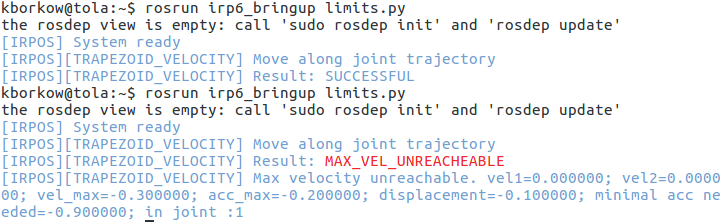
\includegraphics[width=0.8\textwidth]{raport_pics/msgs_from_gen.png}
	\caption{Wiadomości zwrotne otrzymane przy pracy z nowymi funkcjami systemu IRPOS, w~tym jedną z~informacjami o~błędzie i~jego parametrach.}
	\label{}
	\end{figure}
	
	\section{Wiadomości typu \texttt{Trapezoid}}
	\label{sec:msgs}
	Katalog \texttt{orocos\_controllers} został wzbogacony o~dwa nowe katalogi dotyczące przesyłania informacji pomiędzy modułami. Jeden z nich, \texttt{rtt\_trapezoidal\_trajectory\_msgs}, to tylko nakładka pozwalająca używać nowe wiadomości w~OROCOS'owym systemie czasu rzeczywistego. Drugi, \texttt{trapezoidal\_trajectory\_msgs}, zawiera definicje trzech typów wiadomości: 
	\begin{itemize}
	\item \texttt{TrapezoidTrajectory.action}
	\item \texttt{TrapezoidGeneratorGoal.msg}
	\item \texttt{TrapezoidGeneratorResult.msg}
	\end{itemize}
	Pierwsza jest używana do komunikacji z~IRPOS-api, pozostałe są stosowana w~głębszych warstwach systemu. 
	\subsubsection{\texttt{TrapezoidTrajectory.action}}
	\label{sec:msgsact}
	Jak każda wiadomość opierająca się na tzw. \textquotedblleft ROS action protocol\textquotedblright, stworzonym do działania z~wywłaszczanymi zadaniami\cite{ROS}, \texttt{TrapezoidTrajectory.action} dzieli się na trzy części, w~pliku definiującym przedzielone trzema poziomymi kreskami (\textquotedblleft - - -\textquotedblright), które opisuje \hyperref[tab:action]{tablica~1}. Natomiast wszystkie parametry i~ich deskrypcje znajdują się w~\hyperref[tab:actionparams]{tablicy~2}.
	

	\begin{table}[H]
	\label{tab:action}
	\centering
	\begin{tabular}{|m{4em}|m{15em}|m{18em}|}
	 \hline
	 nazwa & ścieżka przesyłu w~IRPOS'ie & opis\\
	 \hline
	 \hline
	 Goal & IRPOS-api $\rightarrow$ komponent akcji & kontener informacji o~specyfikacji żądania od użytkownika i~programisty IRPOS-api \\  
	 \hline
	 Result & komponent akcji $\rightarrow$ IRPOS-api & wynik wykonanych operacji przesyłany  po zakończeniu ruchu \\
	 \hline
	 Feedback & komponent akcji $\rightarrow$ IRPOS-api  & cyklicznie przesyłane wiadomości o~pośrednich wynikach \\
	 \hline
	\end{tabular}
	\caption{Opis części wiadomości typu\textquotedblleft action\textquotedblright}
	\end{table}
	
	\begin{table}[H]
	\label{tab:actionparams}
	\centering
	\begin{tabular}{|m{4em}|m{8em}|m{12em}|m{13em}|}
	\hline
	nazwa części & nazwa & typ danych & opis\\
	\hline
	\hline
	Goal & trajectory & trajectory\_msgs/ JointTrajectory\cite{jtm} & zadana trajektoria (punkty, prędkości i przyśpieszenia końcowe, itp.) \\  
	\cline{2-4}
	& path\_tolerance & control\_msgs/ JointTolerance[]\cite{cmjtm}&tolerancja błędu definiowana dla każdego silnika.\\
	\cline{2-4}
	& research\_mode & bool & flaga trybu badawczego, patrz \hyperref[sec:flags]{3.2.4}\\
	\cline{2-4}
	& duration\_mode & bool & flaga trybu \texttt{duration}, patrz \hyperref[sec:veldurdiff]{3.2.3}\\
	\cline{2-4}
	& save\_data & bool & flaga zapisu danych, patrz \hyperref[sec:flags]{3.2.4}\\
	\cline{2-4}
	& max\_velocities & float64[] & prędkości do osiągnięcia przez silniki, działa tylko w trybie \texttt{velocity}, patrz \hyperref[sec:veldurdiff]{3.2.3}\\
	\cline{2-4}
	& max\_accelerations & float64[] & przyśpieszenia do osiągnięcia przez silniki, działa tylko w trybie \texttt{velocity}, patrz \hyperref[sec:veldurdiff]{3.2.3}\\
	\hline
	Result & result & TrapezoidGeneratorResult & wiadomość tożsama z~tą którą zwraca komponentowi akcji generator, stąd postanowiono użyć jej bezpośrednio; pełna definicja patrz \hyperref[sec:msgsresult]{3.3.3}\\
	\hline
	Feedback & header & Header & nagłówek\\
	\cline{2-4}
	& joint\_names & string[] & używane nazwy silników/stawów\\
	\cline{2-4}
	& desired & trajectory\_msgs/ JointTrajectoryPoint\cite{jtpm} & punkt zadany przez generator\\
	\cline{2-4}
	& actual & trajectory\_msgs/ JointTrajectoryPoint\cite{jtpm} & punkt osiągnięty przez robota\\
	\cline{2-4}
	& error & trajectory\_msgs/ JointTrajectoryPoint\cite{jtpm} & błąd regulacji\\
	\hline
	\end{tabular}
	\caption{Dokładny opis wszystkich zmiennych używanych w~wiadomości \texttt{TrapezoidTrajectory.action}}
	\end{table}
	
	\subsection{\texttt{TrapezoidGeneratorGoal.msg}}
	\label{sec:msgsgoal}
	\texttt{TrapezoidGeneratorGoal.msg} jest zwykłą wiadomością ROS'ową, która przesyłana jest od komponentu akcji do generatora. Jest ona tożsama z~częścią Goal przedstawionej w~\hyperref[tab:actionparams]{tablicy~2}. Rozdzielenie jest pozostałością po wersji, w~której istniało dużo różnić między tymi elementami. 
	\subsection{\texttt{TrapezoidGeneratorResult.msg}}
	\label{sec:msgsresult}
	Wynik ruchu jest sygnalizowany komponentowi akcji przez generator poprzez wysłanie wiadomości typu \texttt{TrapezoidGeneratorResult.msg}. Składa się ona z~ciągu znaków, który jest wypełniony jeśli nastąpił błąd w~trakcie obliczania profilu prędkościowego oraz kodu zwrotnego, którego znaczenie jest zdefiniowane w~tym samym pliku. Pisemna wiadomość została stworzona po to by łatwiej było dobrać nastawy, które będą znajdować się w~przestrzeni mozliwości generatora trapezoidalnego. \hyperref[tab:resultparams]{Tabelica~3} zawiera opis parametrów \texttt{TrapezoidGeneratorResult}, a~\hyperref[tab:resultcodes]{tabelica~4} opis możliwych kodów. Warto wspomnieć, że pierwsze sześć kodów pokrywa się z~używanymi przy generowaniu trajektorii spline'owych. Część \texttt{error\_string} nie występuje wiadomościach stosowanych przez stary generator.
	
	\begin{table}[H]
	\label{tab:resultparams}
	\centering
	\begin{tabular}{|m{12em}|m{12em}|m{13em}|}
	\hline
	nazwa & typ danych & opis\\
	\hline
	\hline
	error\_string & string & dane błędu \\  
	\hline
	error\_code & int32 & kod błędu\\
	\hline
	\end{tabular}
	\caption{Parametry wiadomości \texttt{TrapezoidGeneratorResult}}
	\end{table}	
	
	\begin{table}[H]
	\label{tab:resultcodes}
	\centering
	\begin{tabular}{|m{2em}|m{17 em}|m{18em}|}
	\hline
	kod & nazwa & opis\\
	\hline
	\hline
	0 & SUCCESSFUL & robot osiągnął pożądany cel \\  
	\hline
	-1 & INVALID\_GOAL & co najmniej jeden z~zadanych punktów znajduje się poza przestrzenią osiągalną przez silnik/staw\\
	\hline
	-2 & INVALID\_JOINTS & nazwy silników/stawów lub ich liczba podane w~wiadomości Goal nie pokrywają się z~tymi, które otrzymano z~serwera parametrów\\
	\hline
	-3 & OLD\_HEADER\_TIMESTAMP & błędny czas w~nagłówku\\
	\hline
	-4 & PATH\_TOLERANCE\_VIOLATED & w~trakcie ruchu błąd regulacji jest zbyt duży\\
	\hline
	-5 & GOAL\_TOLERANCE\_VIOLATED & ostateczne położenie jest zbyt daleko od zadanego\\
	\hline
	-6 & INVALID\_LIMIT\_ARRAY & w~trybie prędkościowym podano mniej maksymalnych prędkości i/lub przyśpieszeń, niż jest zadeklarowanych silników/stawów\\
	\hline
	-7 & TRAJECTORY\_NOT\_FEASIBLE & jeden z~warunków trajektorii trapezoidalnej nie został spełniony\\
	\hline
	-8 & CANT\_CALCULATE\_COEFFS & błąd wystąpił przy obliczaniu współczynników profilu prędkościowego\\
	\hline
	-9 & MAX\_VEL\_UNREACHEABLE & w~przypadku zadanych warunków niemożliwe jest osiągnięcie maksymalnej prędkości, patrz \hyperref[sec:flags]{3.2.4}\\
	\hline 
	-10 & BREACHED\_POS\_LIMIT  & zadana trajektoria przechodzi (nie w~miejscu początkowym lub końcowym) przez miejsce wykraczające poza limity silnika/stawu, możliwe tylko gdy prędkość początkowa/końcowa jest większa od tej jaką należy osiągnąć w~fazie bez przyśpieszenia\\
	\hline
	-11 & ACC\_TOO\_SMALL\_FOR\_DURATION & niemożna osiągnąć celu w~zadanym czasie, przy danym przyśpieszeniu maksymalnym\\
	\hline
	-12 & DURATION\_TOO\_LONG & trwanie ruchu zbyt długie, duży skok w~fazie przyśpieszania, występuje przy niektórych prędkościach początkowych/końcowych o~wartości bezwzględnej większej od tej z~fazy zerowego przyśpieszenia\\
	\hline
	-13 & DURATION\_TOO\_SHORT & trwanie ruchu zbyt krótkie, duży skok w~fazie spowalniania, występuje przy niektórych prędkościach początkowych/końcowych o~wartości bezwzględnej większej od tej z~fazy zerowego przyśpieszenia\\
	\hline
	-14 & IMPOSSIBLE\_VELOCITY & prędkość obliczona w~trybie \texttt{duration}, jest o~wartości bezwzględnej większej niż prędkość maksymalna.\\
	\hline
	\end{tabular}
	\caption{Parametry wiadomości \texttt{TrapezoidGeneratorResult}}
	\end{table}	
	
	\section{Nowe komponenty OROCOS}
	Zaimplementowano dwa nowe komponenty OROCOS'owe. Komponent akcji oraz generator trajektorii. Ich kody znajdują się w~katalogu \texttt{orocos\_controllers}. W~tej sekcji wytłumaczone zostanie ich działanie przy użyciu fragmentów kody źródłowego. Drobne zmiany jakie wprowadzono względem oryginalnego kodu (typu deklarowanie, konfiguracja nowych wektorów itp.) zostaną pominięte.
	
	\subsection{Komponent akcji}
	Zaimplementowany w~plikach \texttt{InternalSpaceTrapezoidTrajectoryAction.cpp} \linebreak i~\texttt{InternalSpaceTrapezoidTrajectoryAction.hpp}, rozpoczyna swój cykl życia od zaimportowania kolejnych parametrów z~serwera ROS'owego:
	\begin{itemize}
	\item \texttt{joint\_names}, nazwy silników/stawów w~zależności od przestrzeni pracy;
	\item \texttt{lower\_limits}, dolne położenia możliwe do osiągnięcia przez silniki/stawy;
	\item \texttt{upper\_limits}, górne położenia możliwe do osiągnięcia przez silniki/stawy.
	\end{itemize}
	Zgodnie ze strukturą komponentów OROCOS'owych, działających cyklicznie, moduł ma funkcję \texttt{updateHook} wraz z~dwiema metodami pomocniczymi \texttt{configureHook} oraz \texttt{stratHook}, ich implementacja jest wymagana\cite{orocosbuild}. Obie funkcje konfiguracyjne wywoływane są w~skrypcie \texttt{irp6-p-inside.ops}. Metoda \texttt{configureHook} inicjuje wektory danych do odpowiednich rozmiarów, oraz sprawdza, czy otrzymano odpowiednią liczbę ograniczeń. Natomiast funkcja uruchamiająca pracę komponentu uruchamia serwer akcji, ale ustawia flagę aktywnego celu na \textit{false}, skąd komponent wie, że w~danym momencie nie jest przeprowadzane przetwarzanie celu. Jednakże, by w~pełni móc przedstawić działanie metody \texttt{updateHook}, należy najpierw opisać funkcję \texttt{goalCB}. Jest ona asynchronicznie wywoływana, w~razie odebrania z~wyższej warstwy systemu (IRPOS-api) części \texttt{Goal} z~wiadomości \texttt{TrapezoidTrajectory.action}. Jeśli w~danym momencie jest przetwarzana już jakaś trajektoria nowy cel zostaje odrzucony. W~przeciwnym przypadku 
	komponent wykonuje kolejne czynności:
	\begin{enumerate}
	\item wypełnienie \texttt{remapTable} odpowiedzialnej za zmapowanie nazw podanych w~wiadomości na kolejność nadaną w~serwerze parametrów. W~razie niepowodzenia, czyli niezgodnej liczby nazw silników/stawów, wysyłany jest kod błędu \textit{INVALID\_JOINTS}; 
	\item sprawdzenie czy wszystkie zadane punkty mieszczą się w~ograniczeniach, w wypadku niespełnienia tego warunku w~którymkolwiek punkcie wysyłany jest błąd  \textit{INVALID\_GOAL};
	\item jeśli użytkownik ustawił flagę \texttt{duration\_mode} na \textit{false}, sprawdzona zostaje liczba zadanych prędkości i~przyśpieszeń maksymalnych, niezgodna z~zadeklarowaną liczbą silników/stawów powoduje wysłanie wiadomości o~błędzie \textit{INVALID\_LIMIT\_ARRAY};
	\item na podstawie \texttt{remapTable} zmapowane zostają wszystkie zadane, łącznie z~tablicami ograniczeń kinematycznych;
	\item sprawdzona zostaje poprawność czasu podanego w~nagłówku, błąd wywołuje odesłanie kodu \textit{OLD\_HEADER\_TIMESTAMP};
	\item jeśli uda się połączyć ze wszystkimi komponentami rówieśniczymi wypełniona i~wysłana do generatora zostaje wiadomość typu \texttt{TrapezoidGoal}.
	\end{enumerate}
	Niespełnienie któregokolwiek z~warunków generujących błąd lub problem przy uruchomieniu rówieśników przerywa przetwarzanie wiadomości i~wywołuje odrzucenie zadanego celu. Nowością względem komponentu akcji trajektorii spline'owej jest przetwarzanie maksymalnych prędkości i~przyśpieszeń oraz przepisywanie ich wraz z~flagami. Dla wygody przebudowano stary kod i~przeniesiono jego fragmenty do dedykowanych funkscji.
	\par Metoda \texttt{updateHook} (zgodnie z~ustawieniami z~dnia 30 maja 2018) wywoływana jest co 0.01 sekundy. Zadania jakie kolejno wykonuje to:
	\begin{enumerate}
	\item odczytuje dane o~właściwym i~zadanym położeniu silników/stawów;
	\item sprawdza czy generator zasygnalizował zakończenie wykonywania trajektorii i~reaguje zależnie od otrzymanego wyniku oraz ułożenia robota;
	\item analizuje możliwość przekroczenia tolerancji ścieżki (pomijane w~trybir \texttt{research\_mode});
	\item wysyła część Feedback z~wiadomość typu action.
	\end{enumerate}
	Naturalnie punkt drugi wykonywany będzie  najrzadziej oraz zablokuje wykonywanie kolejnych czynności. Ponad to punkt trzeci i~czwarty zostaną aktywowane tylko jeśli aktywny jest cel oraz otrzymano nowe dane o~konfiguracji robota. Wykrycie przekroczenia ograniczeń ścieżki lub celu skutkuje odesłaniem do użytkownika odpowiedniej wiadomości błędu (patrz TODO) oraz odrzuceniem celu. Wygenerowane informacje o~błędach przy obliczaniu profili prędkościowych powodują tą sama reakcję. Ponownie wprowadzoną zmianą jest przebudowanie kodu, w~tym oddelegowanie części zadań do odpowiedni nazwanych funkcji oraz sposób ustalania zakończenia pracy nad celem (zamiast sprawdzania, czy minął zadany czas ruchu, komponent oczekuje na wiadomość od generatora).
	
	\subsection{Generator trajektorii}
	Kod źródłowy generatora rozłożony jest na dwa pliki: \linebreak \texttt{InternalSpaceTrapezoidTrajectoryGenerator.cpp} i~\texttt{velocityprofile\_trapezoid.cpp} oraz ich pliki nagłówkowe. Jest to zgodne z~konwencją przyjętą dla generatora spline'owego. Komponent \texttt{InternalSpaceTrapezoidTrajectoryGenerator} w~trakcie konfiguracji zwiększa wektor \texttt{vel\_profile\_} zgodnie z~podaną w~parametrach liczbą silników/stawów, co równoważne jest wywołaniu tej samej liczby konstruktorów domyślnych klasy \texttt{velocityprofile\_trapezoid}. Stąd komunikacja między komponentem, a~jego obiektami profili prędkościowych opiera się na wywoływaniu zadanych funkcji i~zwracania wartości, które odpowiadają wiadomościom podanym w~\hyperref[tab:resultcodes]{Tablicy 4}. Wpierw opisane zostanie działanie komponentu, a~następnie jego klasy z~wektora \texttt{vel\_profile\_}. 
	
	\subsubsection{\texttt{InternalSpaceTrapezoidTrajectoryGenerator}}
	Tak samo jak w~przypadku komponentu akcji, konstruktor inicjuje pola klasy wartościami domyślnymi, konfiguruje porty komponentu oraz pobiera kolejne parametry z~serwera ROS'owego:
	\begin{itemize}
	\item \texttt{number\_of\_joints}, liczba silników/stawów;
	\item \texttt{ns\_interval}, parametr tolerancji opóźnień/przyśpieszeń wywołania funkcji \texttt{updateHook};
	\item \texttt{lower\_limits}, dolne położenia możliwe do osiągnięcia przez silniki/stawy;
	\item \texttt{upper\_limits}, górne położenia możliwe do osiągnięcia przez silniki/stawy;
	\item \texttt{max\_velocities}, prędkości maksymalne (obecnie bezpieczne wartości, które po badaniach zostaną zamienione na właściwe);
	\item \texttt{max\_accelerations}, przyśpieszenia maksymalne (obecnie bezpieczne wartości, które po badaniach zostaną zamienione na właściwe).
	\end{itemize}
	\par W~przypadku generatora mamy do czynienie tylko z~czterema funkcjami właściwymi komponentom OROCOS'owym. Są to metody \texttt{*Hook}. Funkcję konfiguracyjną \texttt{cofigureHook} można pokrótce opasać jako inicjalizują porty (\texttt{setDataSample}) oraz zmienne zależne od parametrów pobranych z~serwera. Wywoływana jest ona na etapie przetwarzania skryptu \linebreak\texttt{ipr6-p-inside.opt}. Warto zauważyć, że w~momencie uruchamiania skryptu użytkownika komponent wciąż nie jest gotowy do synchronicznej pracy, bo w~przeciwieństwie do \linebreak\texttt{InternalSpaceTrapezoidTrajectoryAction}, pliki wywoływane przez \texttt{roslaunch \linebreak irp6\_bringup irp6-*-nohardware.launch} nie zawierają komendy start dla niego. Dopiero gdy wywołana zostanie jedna z~metod opisanych na początku~\hyperref[sec:api]{sekcji 4}, poprzez \texttt{connmanSwitch} aktywuje generator. Zapewnia to brak konfliktów między różnymi generatorami, korzystającymi z~tych samych portów. Dopiero teraz metoda \texttt{statrHook} sygnalizuje swoja aktywność przez porty synchronizacji. Zmiany jakie wprowadzono do wyżej wymienionych funkcji są drobne i~polegają na inicjalizacji dodanych pól. 
	\par Najważniejszą częścią komponentu jest metoda \texttt{updateHook}. Każde jej wywołanie pociąga za sobą zasygnalizowanie o~aktywności komponentu oraz sprawdzenie czy nadesłany został nowy cel. Niezależnie od wyniku poprzedniego testu, czyli od tego czy w~danym momencie zmienna zadanych punktów trajektorii pochodzi z~pierwszego odczytu położenia silników/stawów, czy z~obliczeń klas profili prędkościowych, na port zadanych wpisywana jest zawartość wektora \texttt{setpoint\_}. Co więcej przy fladze \texttt{save\_data} ustawionej na \textit{true} przed wysłaniem danych zostaną one zapisane do wektorów-kontenerów. Ze względu na naturę procesów czasu rzeczywistego predefiniowana jest wielkość wektorów, więc przy długim czasie pracy generatora może dojść do niepełnego zapisu. Nadejście nowej wiadomości od komponentu akcji skutkuje przepisaniem danych z~niej do pól obiektu generatora oraz ustawieniem wartości zmiennej \texttt{trajectory\_active\_} na \textit{true}. Ta flaga, obok poprawności nagłówka wiadomości, jest sprawdzana przed rozpoczęciem jakichkolwiek obliczeń. Zachowano z~generatora spline'owego nadpisywanie w~przypadku gdy w~trakcie pracy nad jednym celem przyjdzie nowe żądanie. 
	\par Gdy aktywny jest cel, w~zależności od trybu zdefiniowanego przez użytkownika, uruchamiana jest jedna z~dwóch metod:
	\begin{itemize}
	\item \texttt{updateHookWithVelocityBasedProfiles};
	\item \texttt{updateHookWithDurationBasedProfiles}.
	\end{itemize}
	Ich działanie niewiele różni się od siebie. Postanowiono zastosować oddzielne funkcje ze względu na ewentualne łatwiejsze wprowadzanie oddzielnych, bardziej prawdopodobnych zmian. Schemat działania (uogólniony dla obu trybów) pokazany jest na \hyperref[uHD]{rysunku 2}. Każdy z~kroków przedstawiony na tym schemacie (poza start i~koniec) wiąże się z~wywołaniem podfunkcji. Obliczanie profili prędkościowych wiąże się z~wywołaniem odpowiedniej dla trybu działania metody obiektu klasy \texttt{velocitiprofile\_trapezoid}. Dodatkowo niepowodzenie przy obliczaniu profilu wywołuje wysłanie wiadomości o~niepowodzeniu do komponentu akcji, a~przy fladze \texttt{save\_data} ustawionej na \textit{true} dezaktywacja trajektorii powoduje zapis danych na dysk.
	\begin{figure}[H]
	\centering
	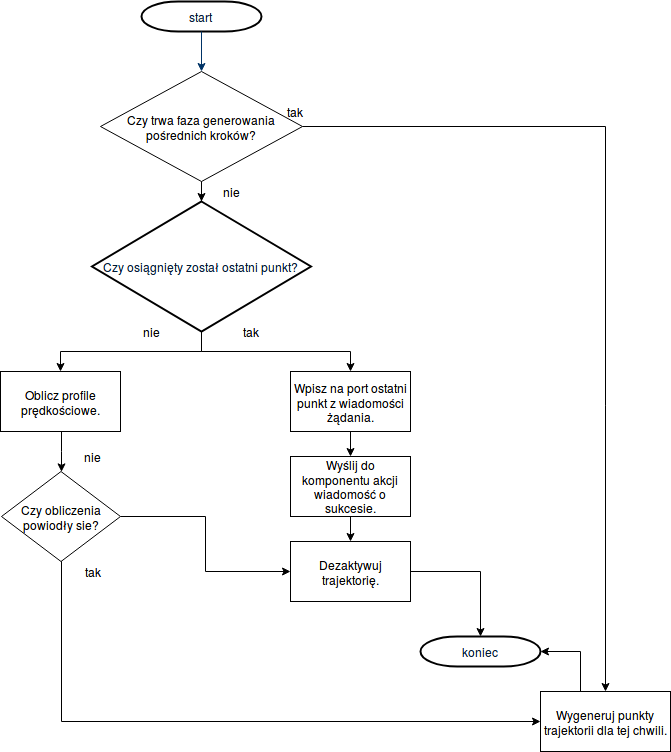
\includegraphics[width=0.9\textwidth]{raport_pics/updateHookDiagram.png}
	\caption{Schemat pracy uogólniony dla obu trybów pracy \texttt{updateHook}.}
	\label{uHD}
	\end{figure}
	\par Różnice pomiędzy działaniem funkcji dla trybu prędkościowego i~czasowego podsumowane są w~\hyperref[tab:modediffUH]{tablicy 5}.
	
	\begin{table}[H]
	\label{tab:modediffUH}
	\centering
	\begin{tabular}{|m{9em}|m{14em}|m{14em}|}
	\hline
	etap & tryb czasowy & tryb prędkościowy\\
	\hline
	\hline
	sprawdzenie czy trwa faza generowania kroków; & testowanie czy minął czas przeznaczony na daną fazę; & testowanie czy wszystkie flagi aktywności silników/stawów ustawione są na \textit{false}; \\  
	\hline
	obliczanie profilu prędkościowego & poprzedzone poszukiwaniem, który z silników/stawów ma do przebycia najdłużej trwającą trasę i~przypisanie tego czasu zadanemu okresowi ruchu dla wszystkich silników/stawów; wykorzystuje metodę \texttt{setProfileDuration} klasy \texttt{velocityprofile\_trapezoid}; & wykorzystuje metodę \texttt{setProfileVelocity} klasy \texttt{velocityprofile\_trapezoid}\\
	\hline
	\end{tabular}
	\caption{Różnice pomiędzy dzianiem funkcji \texttt{updateHook} w~zqależności od ustawionego trybu}
	\end{table}
	\par Komponent, choć wzorowano się na odpowiedniku spline'owym, poza  funkcjami konfiguracyjnymi został stworzony od nowa.
	\subsubsection{\texttt{velocityprofile\_trapezoid}}
	Trzy zadania generatora zostały oddelegowane do klasy \texttt{velocityprofile\_trapezoid}:
	\begin{itemize}
	\item sprawdzenie poprawności żądania;
	\item obliczenie współczynników profilu prędkościowego; 
	\item obliczanie pozycji/prędkości/przyśpieszenia dla danego momentu.
	\end{itemize}
	\hyperref[tab:velProfConds]{Tablica 6} przedstawia jakie warunki muszą zostać spełnione by żądanie zostało uznane za wykonywalne. Odpowiadają one błędom od -7 do -14 z \hyperref[tab:resultcodes]{tablicy 4}.
	\begin{table}[H]
	\label{tab:velProfConds}
	\centering
	\begin{tabular}{|m{10em}|m{8em}|m{22em}|}
	\hline
	warunek & tryb pracy & opis\\
	\hline
	\hline
	$T \geq T_a + T_d$ & czasowy & jeśli trajektoria określana jest na podstawie czasu trwania, przyśpieszenie maksymalne musi być wystarczająco duże by czas fazy przyśpieszenia i~zwalniania łącznie nie przekroczyły czasu trwania ruchu;\\  
	\hline
	$ |v| \leq v_{max} $ & czasowy & obliczona prędkość nie może być większa od maksymalnej\\
	\hline
	$ v_{max} \geq 0 $ & czasowy & ustalono konwencję, wg. której należy podawać prędkości maksymalne jako wartości bezwzględne\\
	\hline
	$ v_{max} > 0 $ & prędkościowy & oprócz konwencji podawania wartości bezwzględnej, warunek ten chroni przed podaniem zera do obliczania czasu trwania ruchu, skutkowałoby to dzieleniem przez zero;\\
	\hline
	$ v_{i} \wedge v_{f} = 0 $ & badawczy & ustalono konwencję, wg. której w~trybie badawczym prędkości skrajne muszą być zerami\\
	\hline
	$ a_{max}h < \frac{|{v_{0}^2} - {v_{0}^2}|}{2} $ & wszystkie & przy dany przyśpieszeniu maksymalnym, dystans może być za krótki by można było go przebyć przy zachowaniu podanych wartości granicznych prędkości;\\
	\hline
	$ T > 0 $ & wszystkie & sprawdzanie przed obliczeniem współczynników, w~tym momencie taki czas trwania sygnalizuje błąd obliczeń; zerowy czas trwania, czyli brak ruchu, powinien zostać wykryty wcześniej;\\
	\hline
	$ T \neq 0 $ & czasowy & czas trwania ruchu musi być większy od zera, jeśli jest równy zeru od razu wysyłana zostaje wiadomość o~dotarciu do celu;\\
	\hline
	$ |s| \geq \varepsilon $ & prędkościowy & droga musi być większa niż ustalona granica błędu położenia, jeśli jest mniejsza od razu wysyłana zostaje wiadomość o~dotarciu do celu;\\
	\hline
	brak skoków trajektorii w~punktach $T_a$ i~$T_d$ & wszystkie & istnieje możliwość, iż przy zadaniu prędkości granicznych większych niż prędkość fazy zerowego przyśpieszenia, nastąpi skok trajektorii w~punktach zmiany fazy; jest to wykrywane po obliczeniu współczynników, dzięki czemu, kilka przypadków takiego określenia prędkości zostaje przyzwolonych;\\
	\hline
	brak przekroczeń położeń granicznych & wszystkie & istnieje możliwość, że przy niezerowych prędkościach granicznych ich osiągnięcie wiąże się z~przejściem przez punkty położone za celem;\\
	\hline
	$ T > T_a + T_d$ & prędkościowy-badawczy & jeśli czas trwania jest równy czasowi trwania faz przyśpieszenia i~spowolnienia nie występuje faza zerowego przyśpieszenia, więc niemożliwe jest zbadanie prędkości maksymalnej;\\
	\hline
	\end{tabular}
	\caption{Warunki realizowalności żądania użytkownika}
	\end{table}
	
	\par Współczynniki profilu prędkościowego obliczane są na podstawie wzorów z~\hyperref[sec:math]{sekcji 2}. Natomiast obliczanie położenia dla danej chwili następuje przy wywołaniu publicznej funkcji przez klasę główną generatora. Przemnażają one współczynniki przez kolejne potęgi podanej chwili $t$.
	
	\section{Testowanie}
	Testowanie generatora rozpoczęto od sprawdzenia, czy działał on przy najprostszych przykładach. Następnie przetestowano wykrywanie nierealizowanych zadanych. Każda próba została poprzedzona oceną zadanych za pomocą skryptów Matlab'owych. Dla funkcji działających w~przestrzeni stawów dodatkowo sprawdzano czy przeniesienie trajektorii do przestrzeni silników nie spowoduje problemów. Wyniki oceniano na podstawie zebranych danych o~położeniach trajektorii wytworzonej przez generator, ostatecznego wyniku pobranego przez IRPOS-api oraz na podstawie obrazu wizualizacji. Każda z~funkcji przedstawionych w~\hyperref[sec:api]{sekcji 5} została przetestowana oddzielnie. Zgodnie z~założeniami przedstawionymi w~\hyperref[sec:borderVels]{sekcji 5.5}, nie testowano nadania prędkości granicznych.
	\subsection{\texttt{move\_to\_motor\_position\_trapezoid\_velocity}}
	Testowanie funkcji działającej w~przestrzeni silników w~trybie prędkościowym.
	\subsubsection{Proste działanie w~trybie niebadawczym}
	\label{sec:MPV}
	Początkowo zadano nastawy, które wymuszały ruch tylko jednego silnika. Podane są w~\hyperref[tab:setup1]{tablicy 7}, każdy wiersz reprezentuje oddzielną symulację. Następnie zastosowano te same nastawy, ale tym razem jednocześnie. W~kolejnym kroku przeprowadzono symulację ruchu w~drugą stronę. 	
	\par Ze względu na liczbę symulacji wykresy z~wynikami pierwszych dwóch testów przedstawiono tylko dla jednego silnika. \hyperref[fig:simpMPVall]{Rysunek 6} jest zbiorem wykresów kolejnych stawów, gdy uruchomiono zmianę położeń z~\hyperref[tab:setup1]{tablicy 7} jednocześnie. Widać na nim, że zgodnie z~założeniami trybu prędkościowego każdy staw kończy poruszanie się w~innym momencie.
	\newpage
	\begin{table}[H]
	\centering
	\begin{tabular}{|m{2.5em}|m{4em}|m{4em}|m{4em}|m{4em}|m{4em}|m{4em}|m{5em}|}
	\hline
	silnik&$ q_i $ & $ q_f $ & $ v_i $ & $ v_f $ & $ v_{max} $ & $ a_{max} $&wynik symulacji\\
	\hline
	\hline
	\hspace{1em}1& 0.0 & 400.0 & 0.0 & 0.0 & 25.0 & 10&\hspace{2em}\checkmark\\ %400.01624549348827
	\hline
	\hspace{1em}2& 0.0 & 100.0 & 0.0 & 0.0 & 35.0 & 20&\hspace{2em}\checkmark\\  %100.06493977550167
	\hline
	\hspace{1em}3& 0.0 & 100.0 & 0.0 & 0.0 & 35.0 & 20&\hspace{2em}\checkmark\\ %100.05074855824355
	\hline
	\hspace{1em}4& 0.0 & 350.0 & 0.0 & 0.0 & 35.0 & 20&\hspace{2em}\checkmark\\  %350.03683107162874
	\hline
	\hspace{1em}5& 0.0 & 400.0 & 0.0 & 0.0 & 35.0 & 20&\hspace{2em}\checkmark\\  %400.0004100112147
	\hline
	\hspace{1em}6& 0.0 & 2000.0 & 0.0 & 0.0 & 35.0 & 20&\hspace{2em}\checkmark\\  %2000.0423718337847
	\hline
	\end{tabular}
	\caption{Wyniki symulacji najprostszego przypadku, badanie oddzielnych silników.}
	\label{tab:setup1}
	\end{table}
	
	\begin{table}[H]
	\centering
	\begin{tabular}{|m{2.5em}|m{4em}|m{4em}|m{4em}|m{4em}|m{4em}|m{4em}|m{5em}|}
	\hline
	silnik&$ q_i $ & $ q_f $ & $ v_i $ & $ v_f $ & $ v_{max} $ & $ a_{max} $&wynik symulacji\\
	\hline
	\hline
	\hspace{1em}1& 0.0 & -400.0 & 0.0 & 0.0 & 25.0 & 10&\hspace{2em}\checkmark\\ %-400.0162154089848
	\hline
	\hspace{1em}2& 0.0 & -100.0 & 0.0 & 0.0 & 35.0 & 20&\hspace{2em}\checkmark\\ %-100.06384704599024
	\hline
	\hspace{1em}3& 0.0 & -70.0 & 0.0 & 0.0 & 35.0 & 20&\hspace{2em}\checkmark\\ %-70.04977729182792
	\hline
	\hspace{1em}4& 0.0 & -60.0 & 0.0 & 0.0 & 35.0 & 20&\hspace{2em}\checkmark\\  %-60.036372838521224
	\hline
	\hspace{1em}5& 0.0 & -70.0 & 0.0 & 0.0 & 35.0 & 20&\hspace{2em}\checkmark\\  %-70.00005703129563
	\hline
	\hspace{1em}6& 0.0 & -900.0 & 0.0 & 0.0 & 35.0 & 20&\hspace{2em}\checkmark\\  %-900.0418019049634
	\hline
	\end{tabular}
	\caption{Wyniki symulacji najprostszego przypadku, badanie oddzielnych silników.}
	\label{tab:setup2}
	\end{table}

	\begin{figure}[H]
		\centering
		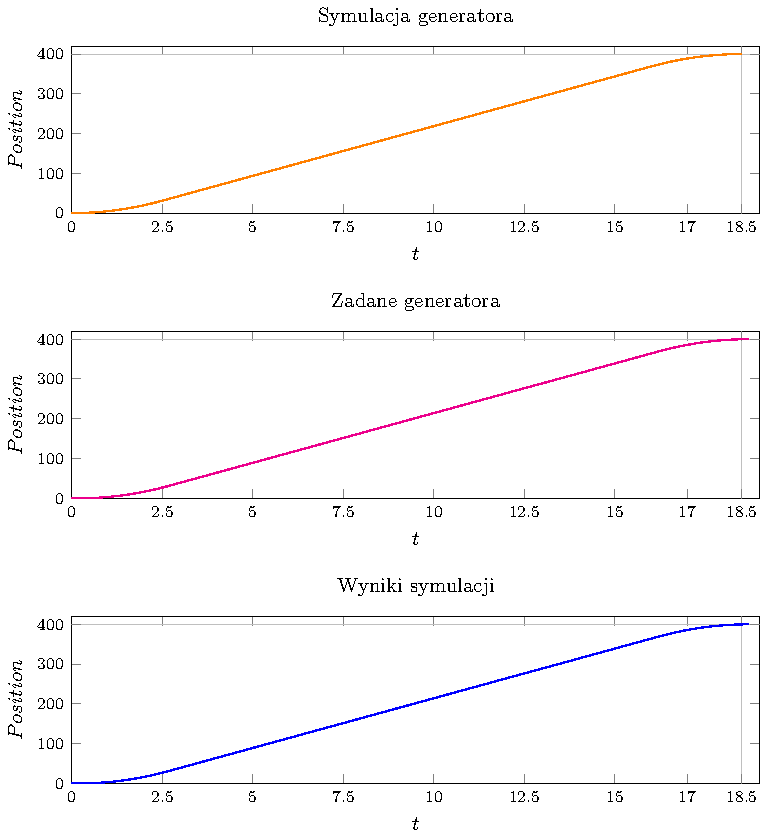
\includegraphics[scale=1.2]{raport_graphs/simpMPV.pdf}
		\caption{Wyniki testu trajektorii dla silnika pierwszego funkcji \texttt{move\_to\_motor\_position\_trapezoid\_velocity} przy nastawach z~\hyperref[tab:setup1]{tablicy 7}.}
		\label{fig:simpMPV}
	\end{figure}


	\begin{figure}[H]
		\centering
		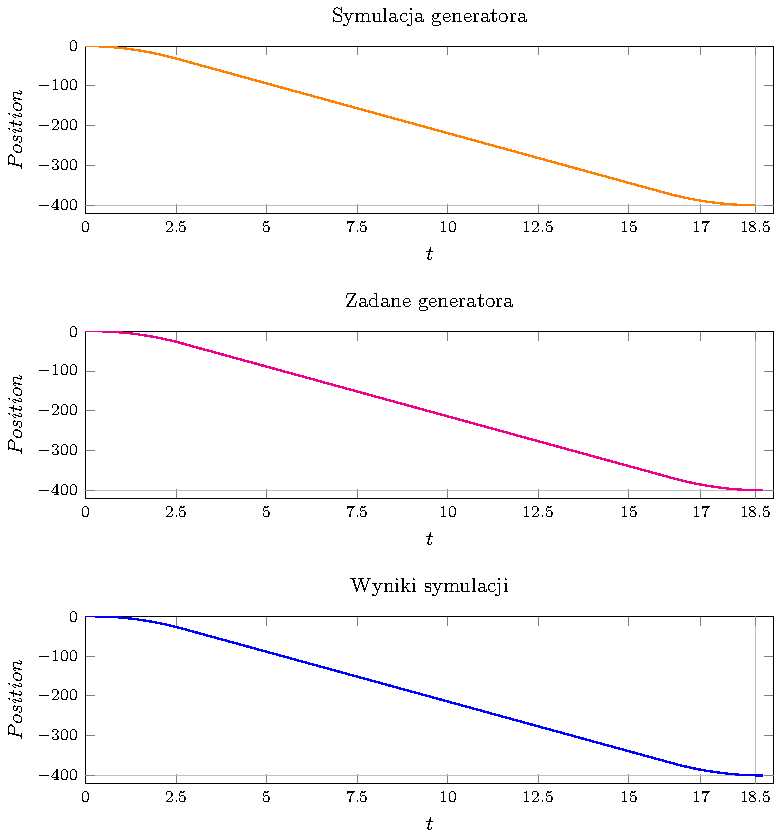
\includegraphics[scale=1.2]{raport_graphs/simpMPVrevers.pdf}
		\caption{Wyniki testu trajektorii dla silnika pierwszego funkcji \texttt{move\_to\_motor\_position\_trapezoid\_velocity} przy nastawach z~\hyperref[tab:setup1]{tablicy 8}.}
		\label{fig:simpMPVrevers}
	\end{figure}
		
	\begin{figure}[H]
		\centering
		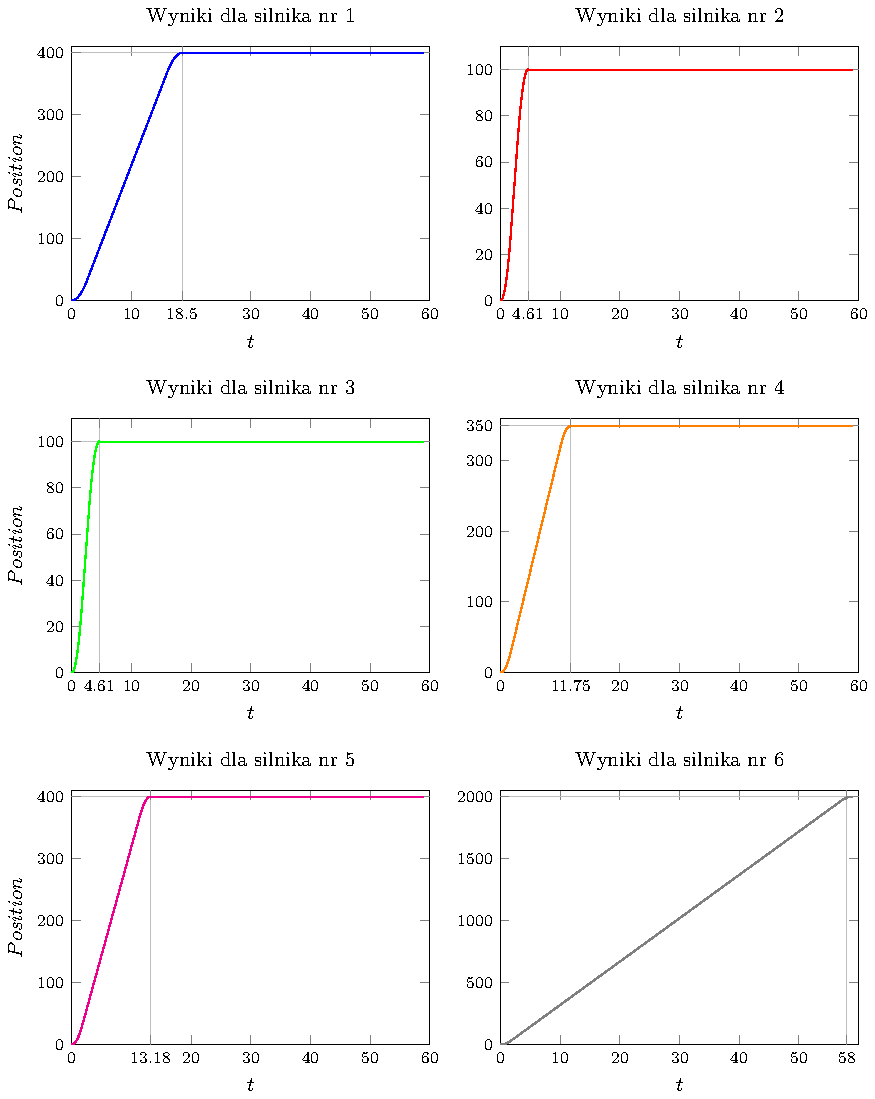
\includegraphics[scale=1.1]{raport_graphs/simpMPVall.pdf}
		\caption{Wyniki testu trajektorii dla silnika pierwszego funkcji \texttt{move\_to\_motor\_position\_trapezoid\_velocity} przy nastawach z~\hyperref[tab:setup1]{tablicy 8}.}
		\label{fig:simpMPVall}
	\end{figure}
		
		%[-470.0, -110.0, -80.0, -70.0, -80.0, -1000.0]
		%[450.0, 100.0, 100.0, 380.0, 490.0, 3000.0]
	\newpage
	\subsubsection{Proste działanie w~trybie badawczym}
	\label{sec:MPVR}
	Porównano wyniki dla z~poprzedniej sekcji, tym razem uruchamiając tryb badawczy. Spodziewano się, że tylko w~przypadku ruchu wstecznego na silniku 4, odległość do przebycia będzie zbyt krótka do osiągnięcia maksymalnej prędkości, ergo odesłana zostanie wiadomość \hyperref[tab:resultcodes]{MAX\_VEL\_UNREACHEABLE}.
	
	\begin{table}[H]
	\centering
	\begin{tabular}{|m{2.5em}|m{4em}|m{4em}|m{4em}|m{4em}|m{4em}|m{4em}|m{5em}|}
	\hline
	silnik&$ q_i $ & $ q_f $ & $ v_i $ & $ v_f $ & $ v_{max} $ & $ a_{max} $&wynik symulacji\\
	\hline
	\hline
	\hspace{1em}1& 0.0 & 400.0 & 0.0 & 0.0 & 25.0 & 10&\hspace{2em}\checkmark\\ %400.0143850928931
	\hline
	\hspace{1em}2& 0.0 & 100.0 & 0.0 & 0.0 & 35.0 & 20&\hspace{2em}\checkmark\\  %100.06486852560562
	\hline
	\hspace{1em}3& 0.0 & 100.0 & 0.0 & 0.0 & 35.0 & 20&\hspace{2em}\checkmark\\ %100.04924828213164
	\hline
	\hspace{1em}4& 0.0 & 350.0 & 0.0 & 0.0 & 35.0 & 20&\hspace{2em}\checkmark\\  %350.03602449535526
	\hline
	\hspace{1em}5& 0.0 & 400.0 & 0.0 & 0.0 & 35.0 & 20&\hspace{2em}\checkmark\\  %400.000206395721
	\hline
	\hspace{1em}6& 0.0 & 2000.0 & 0.0 & 0.0 & 35.0 & 20&\hspace{2em}\checkmark\\  %2000.0292979453866
	\hline
	\end{tabular}
	\caption{Wyniki symulacji najprostszego przypadku, badanie oddzielnych silników. Tryb badawczy.}
	\label{tab:setup3}
	\end{table}
	
	\begin{table}[H]
	\centering
	\begin{tabular}{|m{2.5em}|m{4em}|m{4em}|m{4em}|m{4em}|m{4em}|m{4em}|m{5em}|}
	\hline
	silnik&$ q_i $ & $ q_f $ & $ v_i $ & $ v_f $ & $ v_{max} $ & $ a_{max} $&wynik symulacji\\
	\hline
	\hline
	\hspace{1em}1& 0.0 & -400.0 & 0.0 & 0.0 & 25.0 & 10&\hspace{2em}\checkmark\\ %-400.0144095369332
	\hline
	\hspace{1em}2& 0.0 & -100.0 & 0.0 & 0.0 & 35.0 & 20&\hspace{2em}\checkmark\\ %-100.06421548964671
	\hline
	\hspace{1em}3& 0.0 & -70.0 & 0.0 & 0.0 & 35.0 & 20&\hspace{2em}\checkmark\\ %-70.05025772296632
	\hline
	\hspace{1em}4& 0.0 & -60.0 & 0.0 & 0.0 & 35.0 & 20&\hspace{2em}X\\  %-8.869543149594518e-13
	\hline
	\hspace{1em}5& 0.0 & -70.0 & 0.0 & 0.0 & 35.0 & 20&\hspace{2em}\checkmark\\  %-70.00006451911138
	\hline
	\hspace{1em}6& 0.0 & -900.0 & 0.0 & 0.0 & 35.0 & 20&\hspace{2em}\checkmark\\  %-900.0344946730511
	\hline
	\end{tabular}
	\caption{Wyniki symulacji najprostszego przypadku, badanie oddzielnych silników. Tryb badawczy.}
	\label{tab:setup4}
	\end{table}
	Wyniki uzyskane dla trybu badawczego w~postaci wykresów (\hyperref[fig:simpMPVR]{rysunek 7},\hyperref[fig:simpMPVRrevers]{rysunek 8},\hyperref[fig:simpMPVRall]{rysunek 9}), są tożsame z wynikami z~\hyperref[sec:MPVR]{sekcji 8.1.1}.
	
	\begin{figure}[H]
		\centering
		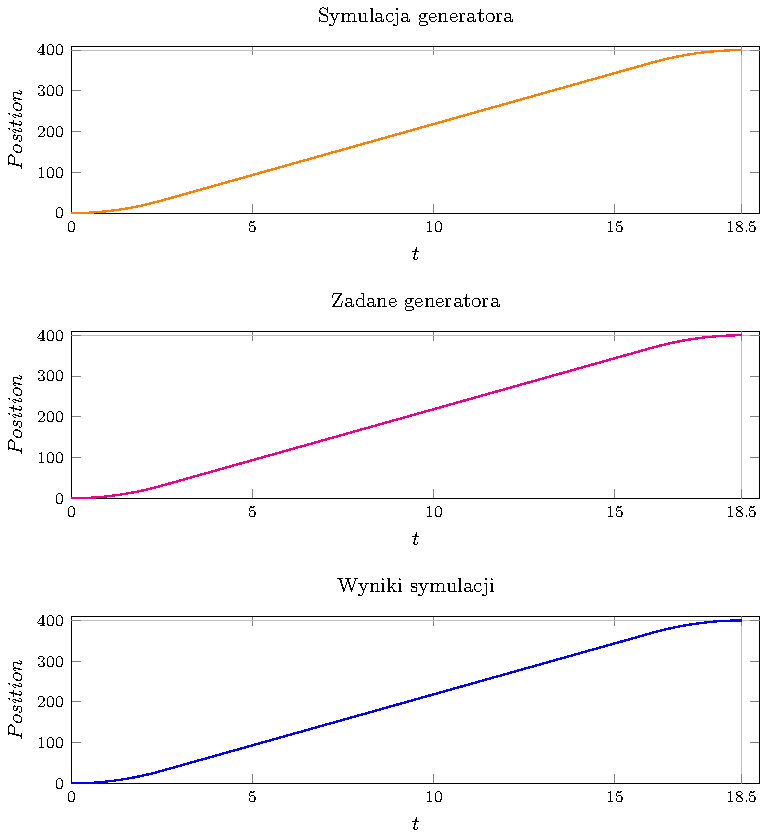
\includegraphics[scale=1.1]{raport_graphs/simpMPVR.pdf}
		\caption{Wyniki testu trajektorii dla silnika pierwszego funkcji \texttt{move\_to\_motor\_position\_trapezoid\_velocity} przy nastawach z~\hyperref[tab:setup3]{tablicy 10}. Tryb badawczy.}
		\label{fig:simpMPVR}
	\end{figure}
	
	\begin{figure}[H]
		\centering
		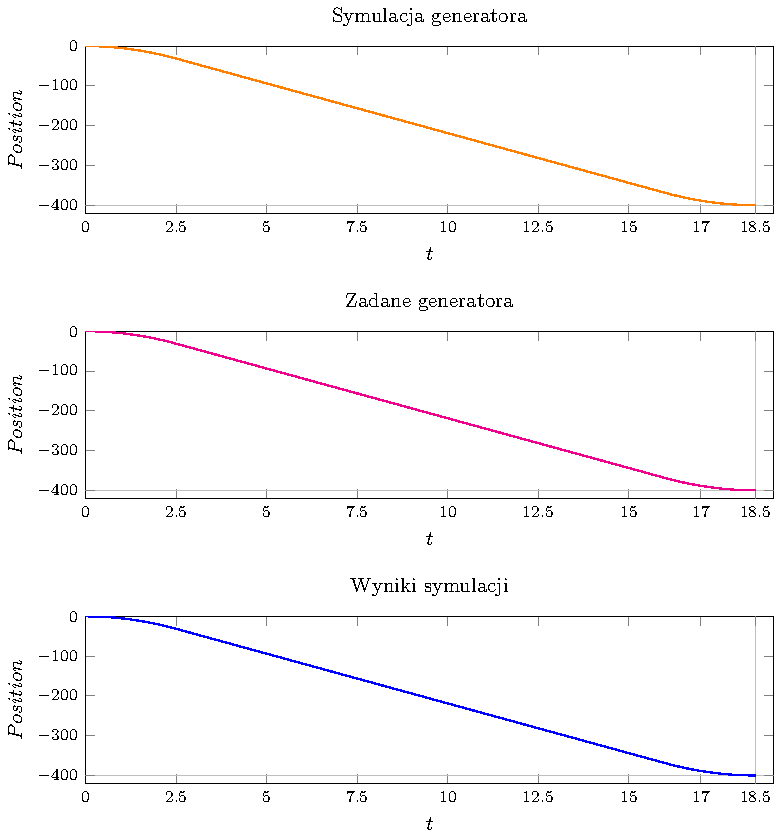
\includegraphics[scale=1.1]{raport_graphs/simpMPVRrevers.pdf}
		\caption{Wyniki testu trajektorii dla silnika pierwszego funkcji \texttt{move\_to\_motor\_position\_trapezoid\_velocity} przy nastawach z~\hyperref[tab:setup4]{tablicy 11}. Tryb badawczy.}
		\label{fig:simpMPVRrevers}
	\end{figure}
	
	\begin{figure}[H]
		\centering
		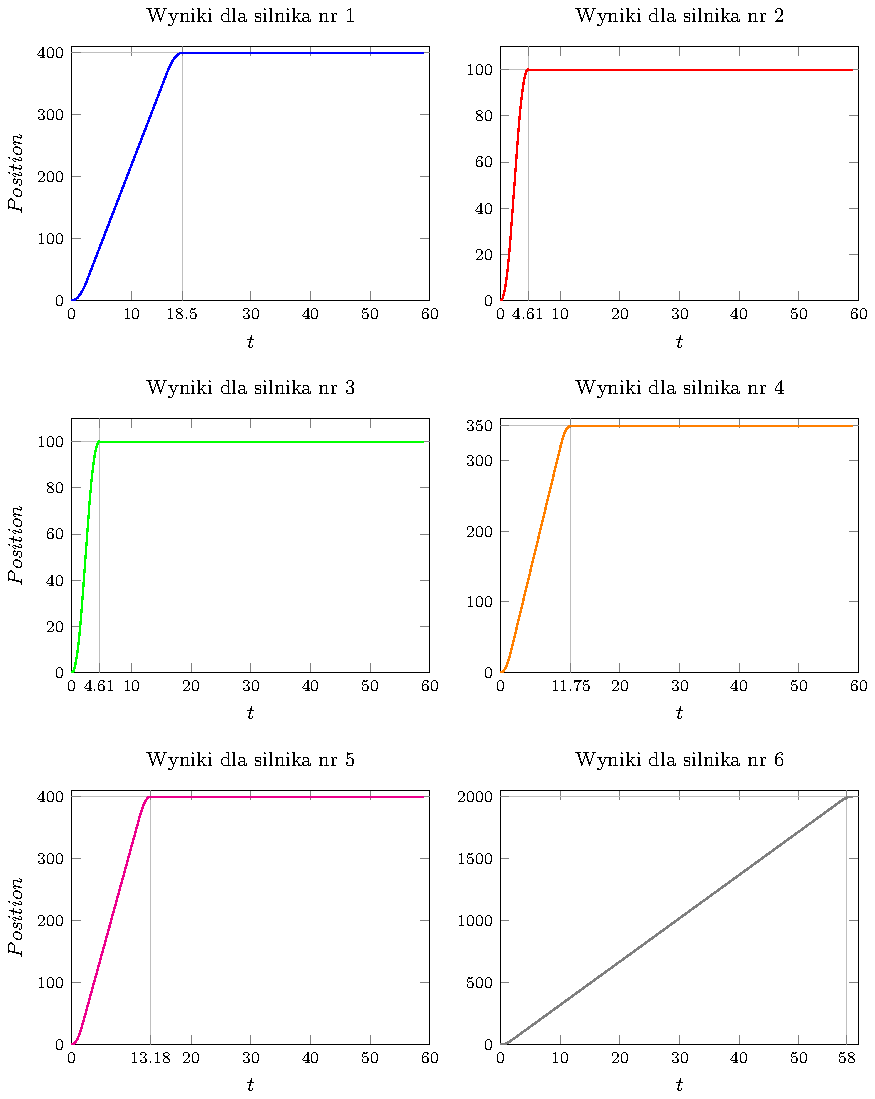
\includegraphics[scale=1.1]{raport_graphs/simpMPVRall.pdf}
		\caption{Wyniki testu trajektorii dla silnika pierwszego funkcji \texttt{move\_to\_motor\_position\_trapezoid\_velocity} przy nastawach z~\hyperref[tab:setup3]{tablicy 10}. Tryb badawczy.}
		\label{fig:simpMPVRall}
	\end{figure}
	
	Jak wspomniano, spodziewano się błędu na silniku 4, przy ruchu $ q_i>q_f$. Takowy otrzymano, co potwierdza \hyperref[fig:res_fail_msg]{rysunek 10} udokumoentowujący go. Warto zaznaczyć, że system numeruje silniki od zera, więc liczba porządkowa jest mniejsza o~jeden.
	
	\begin{figure}[H]
	 	\centering
	 	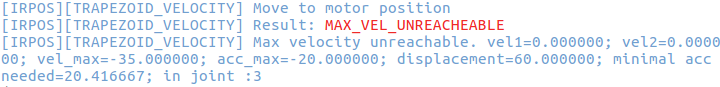
\includegraphics[scale=0.635]{raport_pics/res_fail_msg.png}
	 	\caption{Wyniki testu trajektorii dla silnika pierwszego funkcji \texttt{move\_to\_motor\_position\_trapezoid\_velocity} przy nastawach dla silnika 4~z~\hyperref[tab:setup4]{tablicy~11}. Tryb badawczy.}
		\label{fig:res_fail_msg}
	\end{figure}
	
	Otrzymane wykresy są tożsame z~wykresami otrzymanymi w~sekcji \hyperref[sec:MPV]{8.1.1}, co łącząc z~wynikami ruchu odwrotnego silnika 4, pozwala stwierdzić, że tryb badawczy działa zgodnie z~założeniami. 

	\subsection{\texttt{move\_along\_motor\_trajectory\_trapezoid\_velocity}}
	Testowanie funkcji działającej w~przestrzeni silników w~trybie prędkościowym, pozwalającej na osiągnięcie kilku kolejnych punktów przy jednym wywołaniu funkcji. 
	\subsubsection{Proste działanie w~trybie niebadawczym}
	\label{sec:MTV}
	Ponownie przeprowadzono najpierw badania trajektorii oddzielnie dla każdego silnika, następnie dla wszystkich naraz. Nie przeprowadzano badań oddzielnie dla ruchu $ q_i>q_f $ ze względu na zawarcie ich w~trajektorii zadanej. Zadane przedstawiono w~\hyperref[tab:setup5]{tablicy 11}. Pominięto w~niej prędkości początkowe i~końcowe, które nie podgalają badaniu.
	
	\begin{table}[H]
	\centering
	\begin{tabular}{|m{2.5em}|m{3em}|m{3.5em}|m{3em}|m{3em}|m{3em}|m{4em}|m{3em}|m{5em}|}
	\hline
	silnik&$ q_i $ & $ q_2 $ & $ q_3 $ & $q_4$ & $ q_f $ & $ v_{max} $ & $ a_{max} $&wynik symulacji\\
	\hline
	\hline
	\hspace{1em}1& 0.0 & 400.0 & 200.0 & -200.0 & 100.0 & 25.0 & 10&\hspace{2em}\checkmark\\ %-400.0144095369332
	\hline
	\hspace{1em}2& 0.0 & -100.0 & 100.0 & 20.0 & 0.0 & 35.0 & 20&\hspace{2em}\checkmark\\ %-100.06421548964671
	\hline
	\hspace{1em}3& 0.0 & -70.0 & 50.0 & 0.0 & -30.0 & 35.0 & 20&\hspace{2em}\checkmark\\ %-70.05025772296632
	\hline
	\hspace{1em}4& 0.0 & 350.0 & 100.0 & 200.0 & -50.0 & 35.0 & 20&\hspace{2em}\checkmark\\  %-8.869543149594518e-13
	\hline
	\hspace{1em}5& 0.0 & 400.0 & 0.0 & 0.0 & 100.0 & 35.0 & 20&\hspace{2em}\checkmark\\  %-70.00006451911138
	\hline
	\hspace{1em}6& 0.0 & -1000.0 & -500.0 & 100.0 & 0.0 & 35.0 & 20&\hspace{2em}\checkmark\\  %-900.0344946730511
	\hline
	\end{tabular}
	\caption{Wyniki symulacji najprostszego przypadku, badanie oddzielnych silników.}
	\label{tab:setup5}
	\end{table}	
	
	\begin{figure}[H]
		\centering
		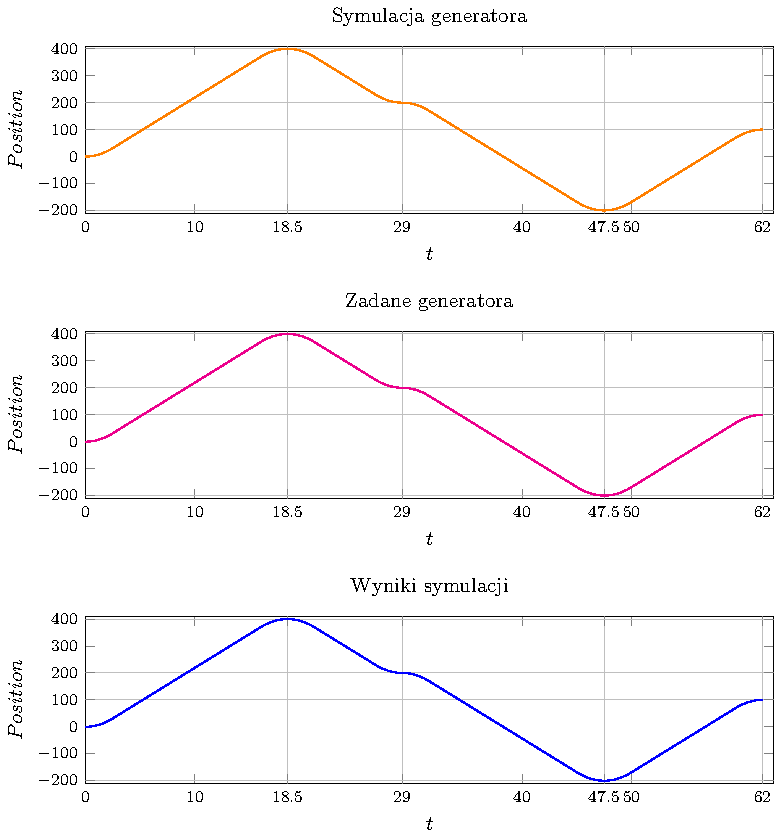
\includegraphics[scale=1.1]{raport_graphs/simpMTV.pdf}
		\caption{Wyniki testu trajektorii dla silnika pierwszego funkcji \texttt{move\_along\_motor\_trajectory\_trapezoid\_velocity} przy nastawach z~\hyperref[tab:setup5]{tablicy 11}.}
		\label{fig:simpMTV}
	\end{figure}
	
	\begin{figure}[H]
		\centering
		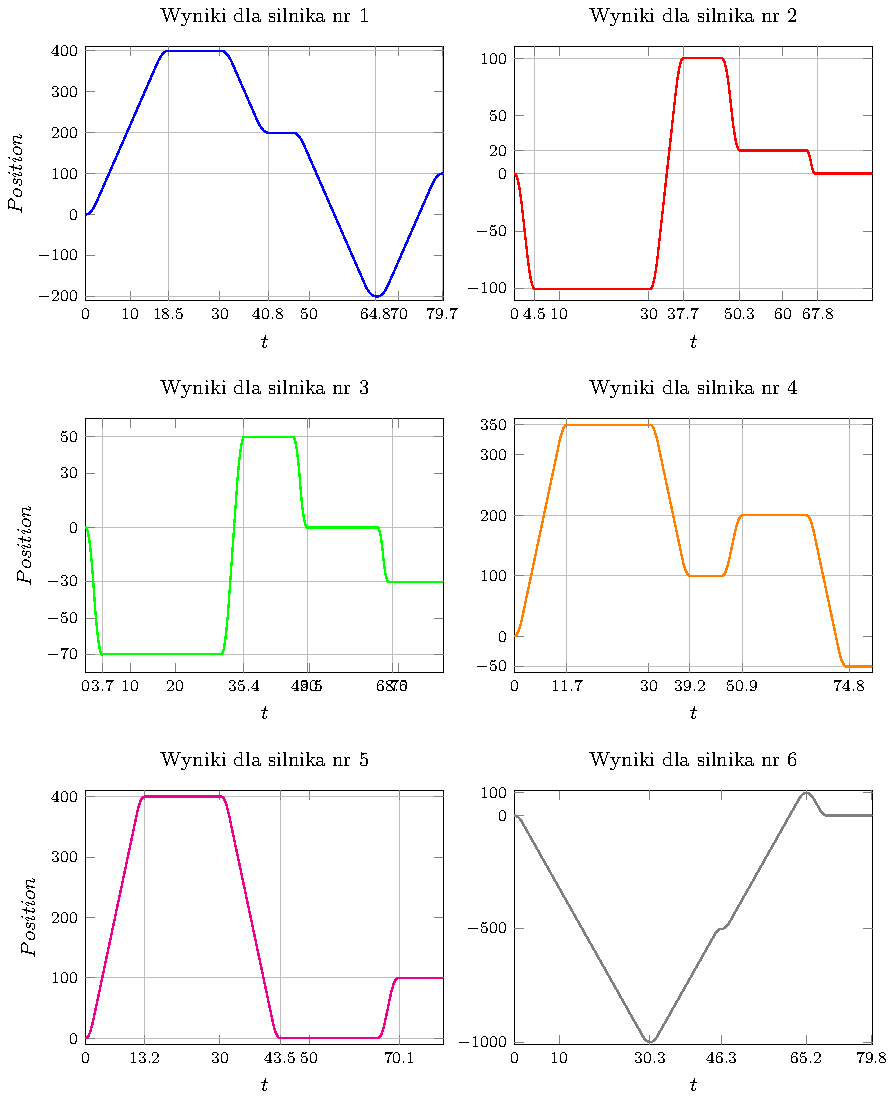
\includegraphics[scale=1.1]{raport_graphs/simpMTVall.pdf}
		\caption{Wyniki testu trajektorii dla wszystkich silników funkcji \texttt{move\_along\_motor\_trajectory\_trapezoid\_velocity} przy nastawach z~\hyperref[tab:setup5]{tablicy 11}.}
		\label{fig:simpMTVall}
	\end{figure}
	
	Jak widać na \hyperref[fig:simpMTVall]{rysunku 12}, silniki "czekają" na siebie. Wizualizują to wypłaszczenia na wykresach. Jest to zgodne z~założeniami generatora. 
	
	\subsubsection{Proste działanie w~trybie badawczym}
	Działanie w~trybie badawczym powinno nie pozwolić na ruch silnika dla nastaw z~\hyperref[tab:setup5]{tablicy 11}, dla silników 2~i~3. 
	
	\begin{figure}[H]
		\centering
		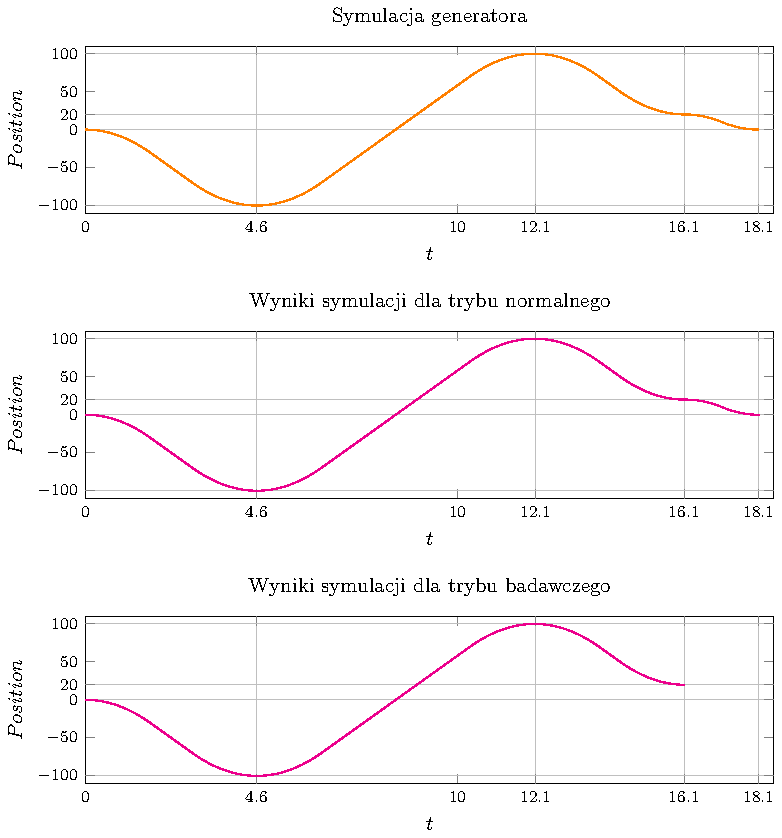
\includegraphics[scale=1.1]{raport_graphs/simpMTVR.pdf}
		\caption{Wyniki testu trajektorii dla trzeciego silnika funkcji \texttt{move\_along\_motor\_trajectory\_trapezoid\_velocity} przy nastawach z~\hyperref[tab:setup5]{tablicy 11}.Tryb badawczy.}		
		\label{fig:simpMTVR}
	\end{figure}
	Rysunek \ref{fig:simpMTVR} pokazuje, różnice pomiędzy trajektorią wygenerowaną w~Matlab'ie, trybem normalnym i~badawczym. Jak się spodziewano tryb badawczy przerwał działanie gdy napotkał problem niemożliwości osiągnięcia maksymalnej prędkości. Jest to zgodne z~założeniami trybu badawczego. Przerwanie pracy następuje nie przed rozpoczęciem całej trajektorii, gdyż zakłada się, że zebranie przynajmniej początkowych danych może być przydatne. Ze względu na alegoryczny wygląd wiadomości błędu do rysunku \ref{fig:res_fail_msg}, pominięto ponowne jego przedstawienie. 
	 
	\begin{figure}[H]
		\centering
		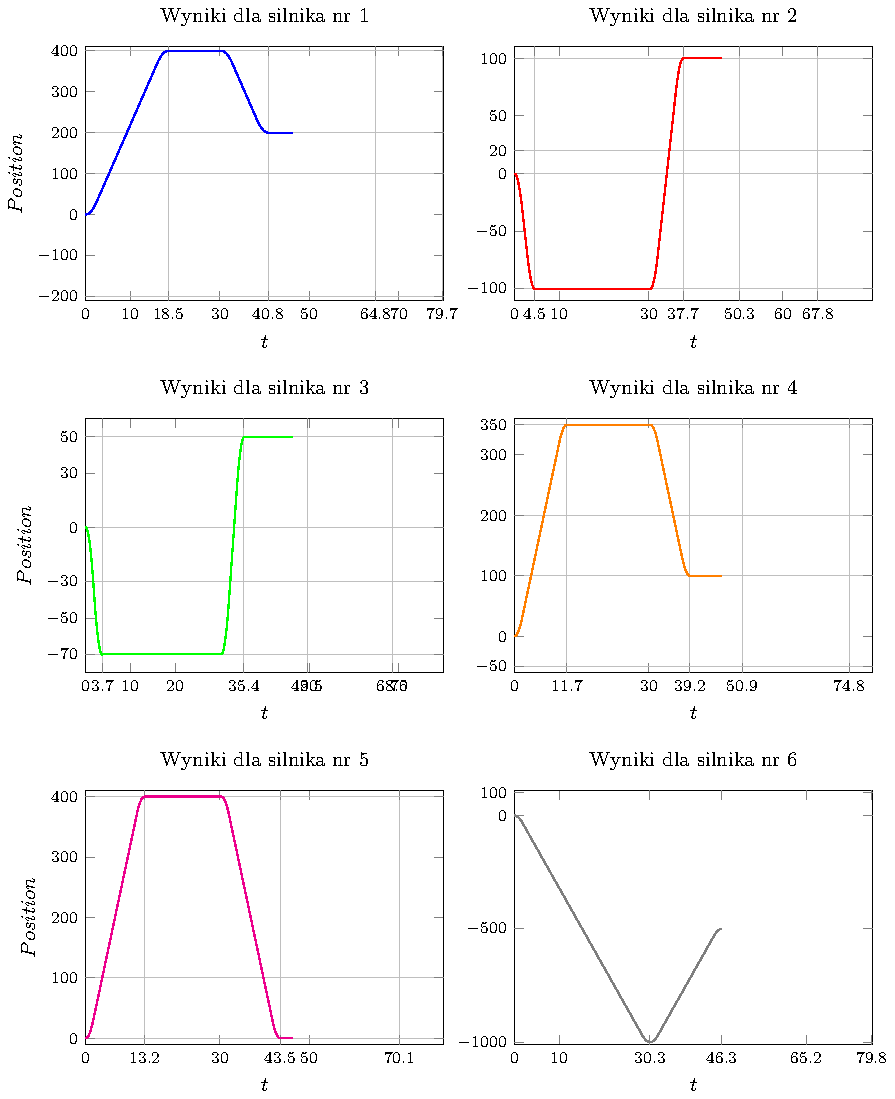
\includegraphics[scale=1.1]{raport_graphs/simpMTVRall.pdf}
		\caption{Wyniki testu trajektorii dla wszystkich silników funkcji \texttt{move\_along\_motor\_trajectory\_trapezoid\_velocity} przy nastawach z~tablicy \ref{tab:setup5}. Tryb badawczy.}		
		\label{fig:simpMTVRall}
	\end{figure}
	
	Na wykresie \ref{fig:simpMTVRall}, szczególnie w porównaniu z~\ref{fig:simpMTVall}, widać moment w~którym generator wykrył błąd zadanych na silniku 2. Tabela \ref{tab:setup6} przedstawia wyniki dla oddzielnego badania trajektorii.
	
	\begin{table}[H]
	\centering
	\begin{tabular}{|m{2.5em}|m{3em}|m{3.5em}|m{3em}|m{3em}|m{3em}|m{4em}|m{3em}|m{5em}|}
	\hline
	silnik&$ q_i $ & $ q_2 $ & $ q_3 $ & $q_4$ & $ q_f $ & $ v_{max} $ & $ a_{max} $&wynik symulacji\\
	\hline
	\hline
	\hspace{1em}1& 0.0 & 400.0 & 200.0 & -200.0 & 100.0 & 25.0 & 10&\hspace{2em}\checkmark\\ %-400.0144095369332
	\hline
	\hspace{1em}2& 0.0 & -100.0 & 100.0 & 20.0 & 0.0 & 35.0 & 20&\hspace{2em}\checkmark\\ %-100.06421548964671
	\hline
	\hspace{1em}3& 0.0 & -70.0 & 50.0 & 0.0 & -30.0 & 35.0 & 20&\hspace{2em}\checkmark\\ %-70.05025772296632
	\hline
	\hspace{1em}4& 0.0 & 350.0 & 100.0 & 200.0 & -50.0 & 35.0 & 20&\hspace{2em}\checkmark\\  %-8.869543149594518e-13
	\hline
	\hspace{1em}5& 0.0 & 400.0 & 0.0 & 0.0 & 100.0 & 35.0 & 20&\hspace{2em}\checkmark\\  %-70.00006451911138
	\hline
	\hspace{1em}6& 0.0 & -1000.0 & -500.0 & 100.0 & 0.0 & 35.0 & 20&\hspace{2em}\checkmark\\  %-900.0344946730511
	\hline
	\end{tabular}
	\caption{Wyniki symulacji najprostszego przypadku, badanie oddzielnych silników. Tryb badawczy.}
	\label{tab:setup6}
	\end{table}	
	
	\subsection{\texttt{move\_to\_motor\_position\_trapezoid\_duration}}
	Testowanie funkcji działającej w~przestrzeni silników w~trybie czasowym.
	\subsubsection{Proste działanie w~trybie niebadawczym}
	Wykonano testy analogiczne do tych z~sekcji \ref{sec:MPV}. Wyniki przedstawiono w~tabelach \ref{tab:setup7} i~\ref{tab:setup8} oraz  na wykresach \ref{fig:simpMPD}, \ref{fig:simpMPDrevers} i~\ref{fig:simpMPDall}. Warto zauważyć, że wywołanie funkcji, nie zawiera nadania prędkości i~przyśpieszenia maksymalnego. Podane w tabelach wartości są wpisane do plików konfiguracyjnych.

	\begin{table}[H]
	\centering
	\begin{tabular}{|m{2.5em}|m{4em}|m{4em}|m{4em}|m{4em}|m{4em}|m{4em}|m{5em}|}
	\hline
	silnik&$ q_i $ & $ q_f $ & $ v_i $ & $ v_f $ & $ v_{max} $ & $ a_{max} $&wynik symulacji\\
	\hline
	\hline
	\hspace{1em}1& 0.0 & 400.0 & 0.0 & 0.0 & 20.0 & 10&\hspace{2em}\checkmark\\ %400.01624549348827
	\hline
	\hspace{1em}2& 0.0 & 100.0 & 0.0 & 0.0 & 20.0 & 10&\hspace{2em}\checkmark\\  %100.06493977550167
	\hline
	\hspace{1em}3& 0.0 & 100.0 & 0.0 & 0.0 & 20.0 & 10&\hspace{2em}\checkmark\\ %100.05074855824355
	\hline
	\hspace{1em}4& 0.0 & 350.0 & 0.0 & 0.0 & 20.0 & 10&\hspace{2em}\checkmark\\  %350.03683107162874
	\hline
	\hspace{1em}5& 0.0 & 400.0 & 0.0 & 0.0 & 20.0 & 10&\hspace{2em}\checkmark\\  %400.0004100112147
	\hline
	\hspace{1em}6& 0.0 & 2000.0 & 0.0 & 0.0 & 20.0 & 10&\hspace{2em}\checkmark\\  %2000.0423718337847
	\hline
	\end{tabular}
	\caption{Wyniki symulacji najprostszego przypadku, badanie oddzielnych silników.}
	\label{tab:setup7}
	\end{table}
	
	\begin{table}[H]
	\centering
	\begin{tabular}{|m{2.5em}|m{4em}|m{4em}|m{4em}|m{4em}|m{4em}|m{4em}|m{5em}|}
	\hline
	silnik&$ q_i $ & $ q_f $ & $ v_i $ & $ v_f $ & $ v_{max} $ & $ a_{max} $&wynik symulacji\\
	\hline
	\hline
	\hspace{1em}1& 0.0 & -400.0 & 0.0 & 0.0 & 20.0 & 10&\hspace{2em}\checkmark\\ %-400.0162154089848
	\hline
	\hspace{1em}2& 0.0 & -100.0 & 0.0 & 0.0 & 20.0 & 10&\hspace{2em}\checkmark\\ %-100.06384704599024
	\hline
	\hspace{1em}3& 0.0 & -70.0 & 0.0 & 0.0 & 20.0 & 10&\hspace{2em}\checkmark\\ %-70.04977729182792
	\hline
	\hspace{1em}4& 0.0 & -60.0 & 0.0 & 0.0 & 20.0 & 10&\hspace{2em}\checkmark\\  %-60.036372838521224
	\hline
	\hspace{1em}5& 0.0 & -70.0 & 0.0 & 0.0 & 20.0 & 10&\hspace{2em}\checkmark\\  %-70.00005703129563
	\hline
	\hspace{1em}6& 0.0 & -900.0 & 0.0 & 0.0 & 20.0 & 10&\hspace{2em}\checkmark\\  %-900.0418019049634
	\hline
	\end{tabular}
	\caption{Wyniki symulacji najprostszego przypadku, badanie oddzielnych silników.}
	\label{tab:setup8}
	\end{table}

	\begin{figure}[H]
		\centering
		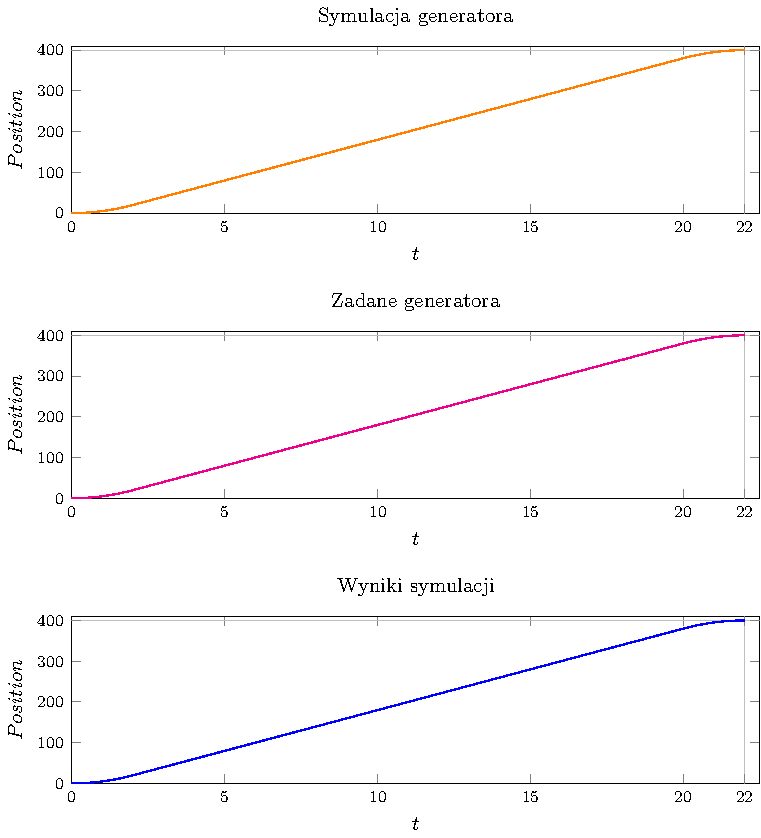
\includegraphics[scale=1.2]{raport_graphs/simpMPD.pdf}
		\caption{Wyniki testu trajektorii dla silnika pierwszego funkcji \texttt{move\_to\_motor\_position\_trapezoid\_duration} przy nastawach z~tablicy \ref{tab:setup7}.}
		\label{fig:simpMPD}
	\end{figure}


	\begin{figure}[H]
		\centering
		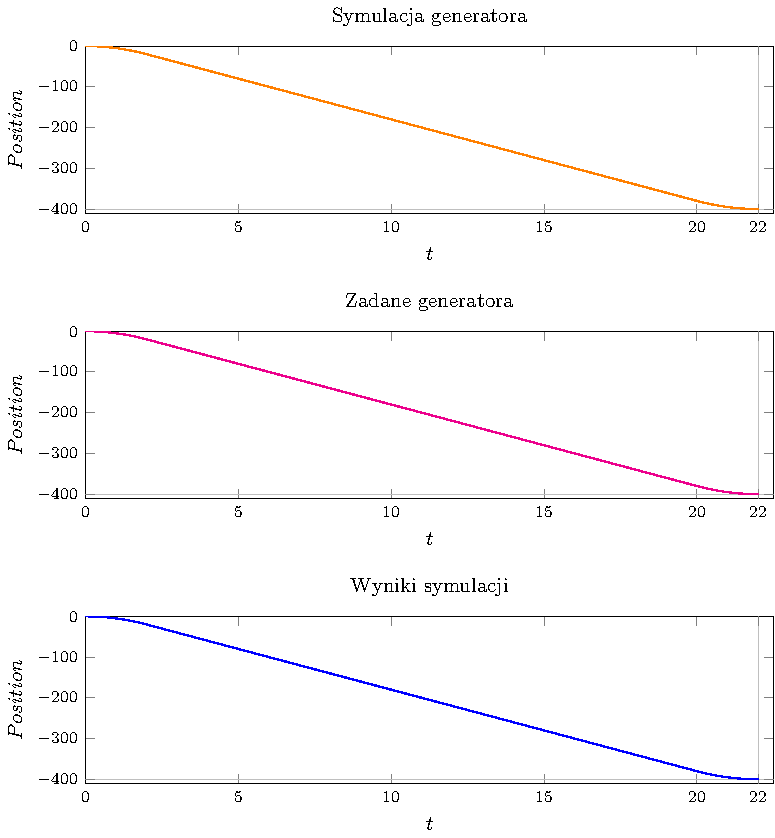
\includegraphics[scale=1.2]{raport_graphs/simpMPDrevers.pdf}
		\caption{Wyniki testu trajektorii dla silnika pierwszego funkcji \texttt{move\_to\_motor\_position\_trapezoid\_duration} przy nastawach z~tablicy \ref{tab:setup8}.}
		\label{fig:simpMPDrevers}
	\end{figure}
		
	\begin{figure}[H]
		\centering
		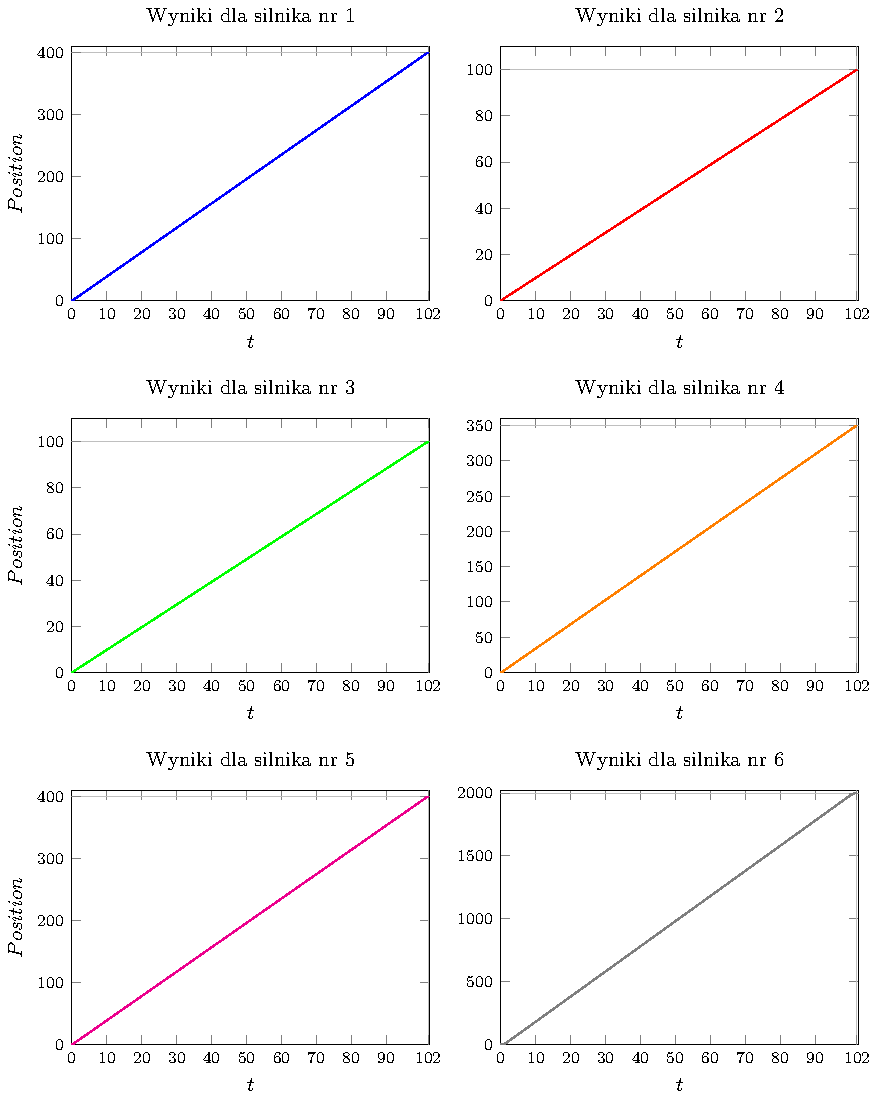
\includegraphics[scale=1.1]{raport_graphs/simpMPDall.pdf}
		\caption{Wyniki testu trajektorii dla silnika pierwszego funkcji \texttt{move\_to\_motor\_position\_trapezoid\_duration} przy nastawach z~tablicy \ref{tab:setup7}.}
		\label{fig:simpMPDall}
	\end{figure}	
	
	Ważnym jest by zwrócić uwagę na fakt, że w~trybie czasowym wszystkie silniki pracują tak samo długo (patrz rysunek \ref{fig:simpMPDall}).
	
	\subsubsection{Proste działanie w~trybie badawczym}
	Zgodnie z~sekcją \ref{sec:flags} nie spodziewana jest żadna różnica pomiędzy pracą funkcji w~trybie normalnym i~badawczym. Spowodowane jest to niebadaniem prędkości początkowych/końcowych, które były by zakazane oraz faktem, że tryb czasowy nie został stworzony do celu badania właściwości kinematycznych robota. 
	Zadane dla ruchu są tożsame z~podanymi w~tabelach \ref{tab:setup7} oraz \ref{tab:setup8}. Wyniki badania podane, przedstawione na wykresach \ref{fig:simpMPDR},\ref{fig:simpMPDRrevers} oraz \ref{fig:simpMPDRall}, potwierdzają poprawne działanie funkcji.
	
	\begin{table}[H]
	\centering
	\begin{tabular}{|m{2.5em}|m{4em}|m{4em}|m{4em}|m{4em}|m{4em}|m{4em}|m{5em}|}
	\hline
	silnik&$ q_i $ & $ q_f $ & $ v_i $ & $ v_f $ & $ v_{max} $ & $ a_{max} $&wynik symulacji\\
	\hline
	\hline
	\hspace{1em}1& 0.0 & 400.0 & 0.0 & 0.0 & 20.0 & 10&\hspace{2em}\checkmark\\ %400.01624549348827
	\hline
	\hspace{1em}2& 0.0 & 100.0 & 0.0 & 0.0 & 20.0 & 10&\hspace{2em}\checkmark\\  %100.06493977550167
	\hline
	\hspace{1em}3& 0.0 & 100.0 & 0.0 & 0.0 & 20.0 & 10&\hspace{2em}\checkmark\\ %100.05074855824355
	\hline
	\hspace{1em}4& 0.0 & 350.0 & 0.0 & 0.0 & 20.0 & 10&\hspace{2em}\checkmark\\  %350.03683107162874
	\hline
	\hspace{1em}5& 0.0 & 400.0 & 0.0 & 0.0 & 20.0 & 10&\hspace{2em}\checkmark\\  %400.0004100112147
	\hline
	\hspace{1em}6& 0.0 & 2000.0 & 0.0 & 0.0 & 20.0 & 10&\hspace{2em}\checkmark\\  %2000.0423718337847
	\hline
	\end{tabular}
	\caption{Wyniki symulacji najprostszego przypadku, badanie oddzielnych silników.}
	\label{tab:setup9}
	\end{table}
	
	\begin{table}[H]
	\centering
	\begin{tabular}{|m{2.5em}|m{4em}|m{4em}|m{4em}|m{4em}|m{4em}|m{4em}|m{5em}|}
	\hline
	silnik&$ q_i $ & $ q_f $ & $ v_i $ & $ v_f $ & $ v_{max} $ & $ a_{max} $&wynik symulacji\\
	\hline
	\hline
	\hspace{1em}1& 0.0 & -400.0 & 0.0 & 0.0 & 20.0 & 10&\hspace{2em}\checkmark\\ %-400.0162154089848
	\hline
	\hspace{1em}2& 0.0 & -100.0 & 0.0 & 0.0 & 20.0 & 10&\hspace{2em}\checkmark\\ %-100.06384704599024
	\hline
	\hspace{1em}3& 0.0 & -70.0 & 0.0 & 0.0 & 20.0 & 10&\hspace{2em}\checkmark\\ %-70.04977729182792
	\hline
	\hspace{1em}4& 0.0 & -60.0 & 0.0 & 0.0 & 20.0 & 10&\hspace{2em}\checkmark\\  %-60.036372838521224
	\hline
	\hspace{1em}5& 0.0 & -70.0 & 0.0 & 0.0 & 20.0 & 10&\hspace{2em}\checkmark\\  %-70.00005703129563
	\hline
	\hspace{1em}6& 0.0 & -900.0 & 0.0 & 0.0 & 20.0 & 10&\hspace{2em}\checkmark\\  %-900.0418019049634
	\hline
	\end{tabular}
	\caption{Wyniki symulacji najprostszego przypadku, badanie oddzielnych silników.}
	\label{tab:setup10}
	\end{table}
	
	\begin{figure}[H]
		\centering
		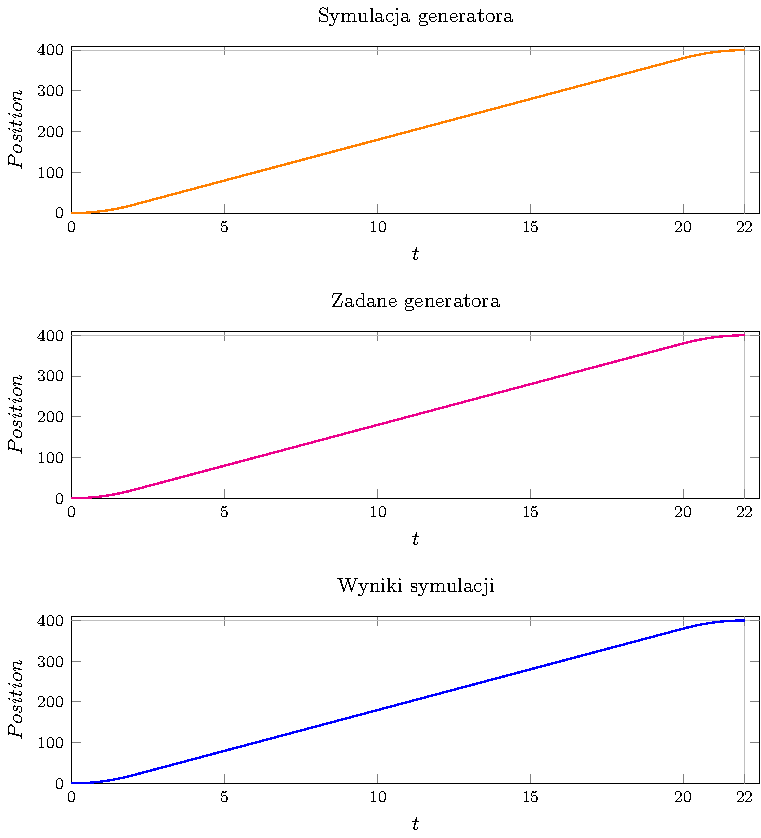
\includegraphics[scale=1.2]{raport_graphs/simpMPDR.pdf}
		\caption{Wyniki testu trajektorii dla silnika pierwszego funkcji \texttt{move\_to\_motor\_position\_trapezoid\_duration} przy nastawach z~tablicy \ref{tab:setup9}. Tryb badawczy.}
		\label{fig:simpMPDR}
	\end{figure}

	\begin{figure}[H]
		\centering
		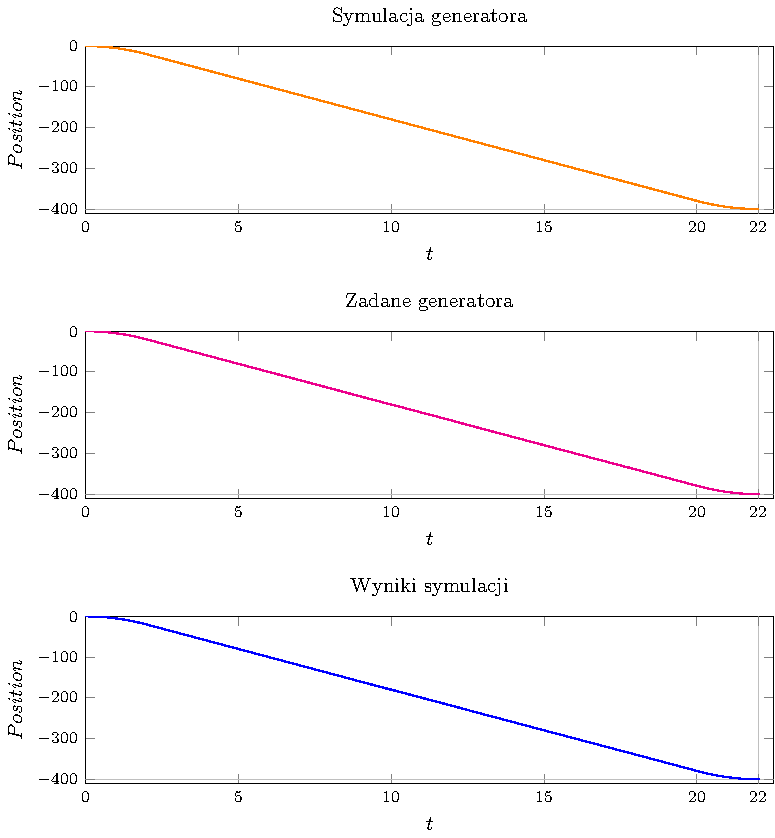
\includegraphics[scale=1.2]{raport_graphs/simpMPDRrevers.pdf}
		\caption{Wyniki testu trajektorii dla silnika pierwszego funkcji \texttt{move\_to\_motor\_position\_trapezoid\_duration} przy nastawach z~tablicy \ref{tab:setup10}. Tryb badawczy.}
		\label{fig:simpMPDRrevers}
	\end{figure}
		
	\begin{figure}[H]
		\centering
		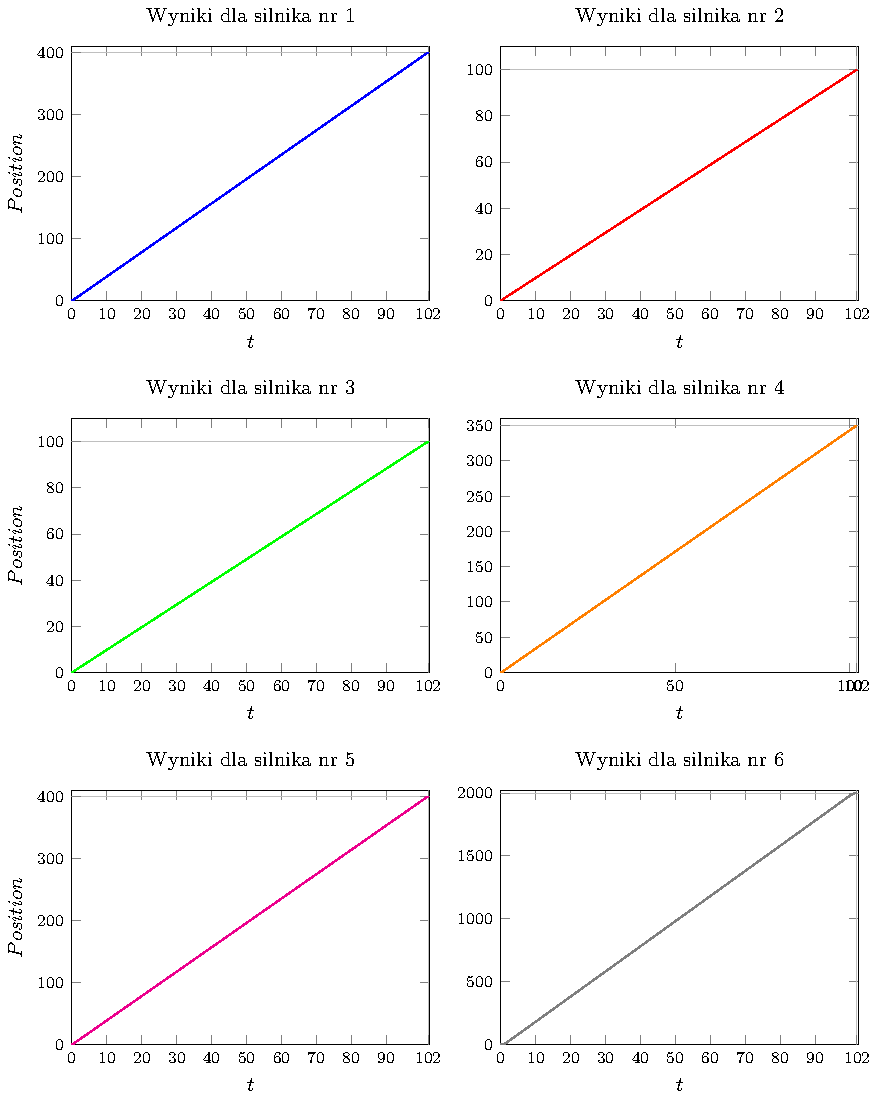
\includegraphics[scale=1.1]{raport_graphs/simpMPDRall.pdf}
		\caption{Wyniki testu trajektorii dla silnika pierwszego funkcji \texttt{move\_to\_motor\_position\_trapezoid\_duration} przy nastawach z~tablicy \ref{tab:setup9}. Tryb badawczy.}
		\label{fig:simpMPDRall}
	\end{figure}	
	
	\subsection{\texttt{move\_along\_motor\_trajectory\_trapezoid\_duration}}
	
	Testowanie funkcji działającej w~przestrzeni silników w~trybie czasowym, pozwalającej na osiągnięcie kilku kolejnych punktów przy jednym wywołaniu funkcji. 

	\subsubsection{Proste działanie w~trybie niebadawczym}
	Ponowiono badania funkcji zadającej całą trajektorię, nadając punkty do osiągnięcia podane w~tablicy \ref{fig:setup11}, zarówno dla każdego silnika oddzielnie, jak i~dla wszystkich naraz.
	
	\begin{table}[H]
	\centering
	\begin{tabular}{|m{2.5em}|m{3em}|m{3.5em}|m{3em}|m{3em}|m{3em}|m{4em}|m{3em}|m{5em}|}
	\hline
	silnik&$ q_i $ & $ q_2 $ & $ q_3 $ & $q_4$ & $ q_f $ & $ v_{max} $ & $ a_{max} $&wynik symulacji\\
	\hline
	\hline
	\hspace{1em}1& 0.0 & 400.0 & 200.0 & -200.0 & 100.0 & 20.0 & 10&\hspace{2em}\checkmark\\ %-400.0144095369332
	\hline
	\hspace{1em}2& 0.0 & -100.0 & 100.0 & 20.0 & 0.0 & 20.0 & 10&\hspace{2em}\checkmark\\ %-100.06421548964671
	\hline
	\hspace{1em}3& 0.0 & -70.0 & 50.0 & 0.0 & -30.0 & 20.0 & 10&\hspace{2em}\checkmark\\ %-70.05025772296632
	\hline
	\hspace{1em}4& 0.0 & 350.0 & 100.0 & 200.0 & -50.0 & 20.0 & 10&\hspace{2em}\checkmark\\  %-8.869543149594518e-13
	\hline
	\hspace{1em}5& 0.0 & 400.0 & 0.0 & 0.0 & 100.0 & 20.0 & 10&\hspace{2em}\checkmark\\  %-70.00006451911138
	\hline
	\hspace{1em}6& 0.0 & -1000.0 & -500.0 & 100.0 & 0.0 & 20.0 & 10&\hspace{2em}\checkmark\\  %-900.0344946730511
	\hline
	\end{tabular}
	\caption{Wyniki symulacji najprostszego przypadku, badanie oddzielnych silników.}
	\label{tab:setup11}
	\end{table}	
	
	\begin{figure}[H]
		\centering
		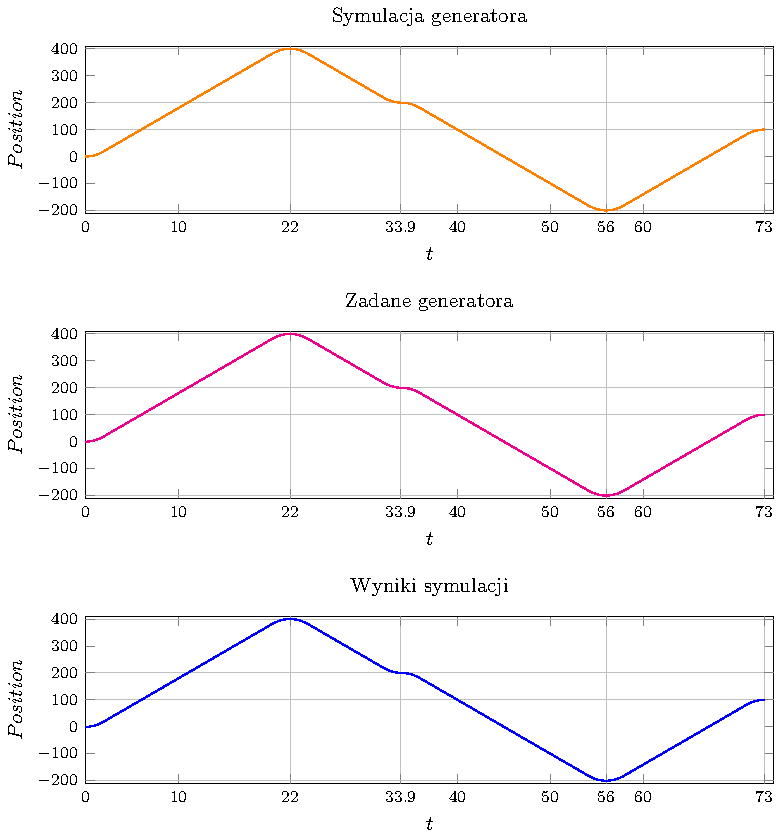
\includegraphics[scale=1.1]{raport_graphs/simpMTD.pdf}
		\caption{Wyniki testu trajektorii dla silnika pierwszego funkcji \texttt{move\_along\_motor\_trajectory\_trapezoid\_duration} przy nastawach z~tablicy \ref{tab:setup11}.}
		\label{fig:simpMTD}
	\end{figure}
	
	Wykresy zgodnie z~przewidywaniem nie różnią się od tych z~rysunku \ref{fig:simpMTV}, gdyż nie ma czasu oczekiwania na pozostałe silniki.
	
	\begin{figure}[H]
		\centering
		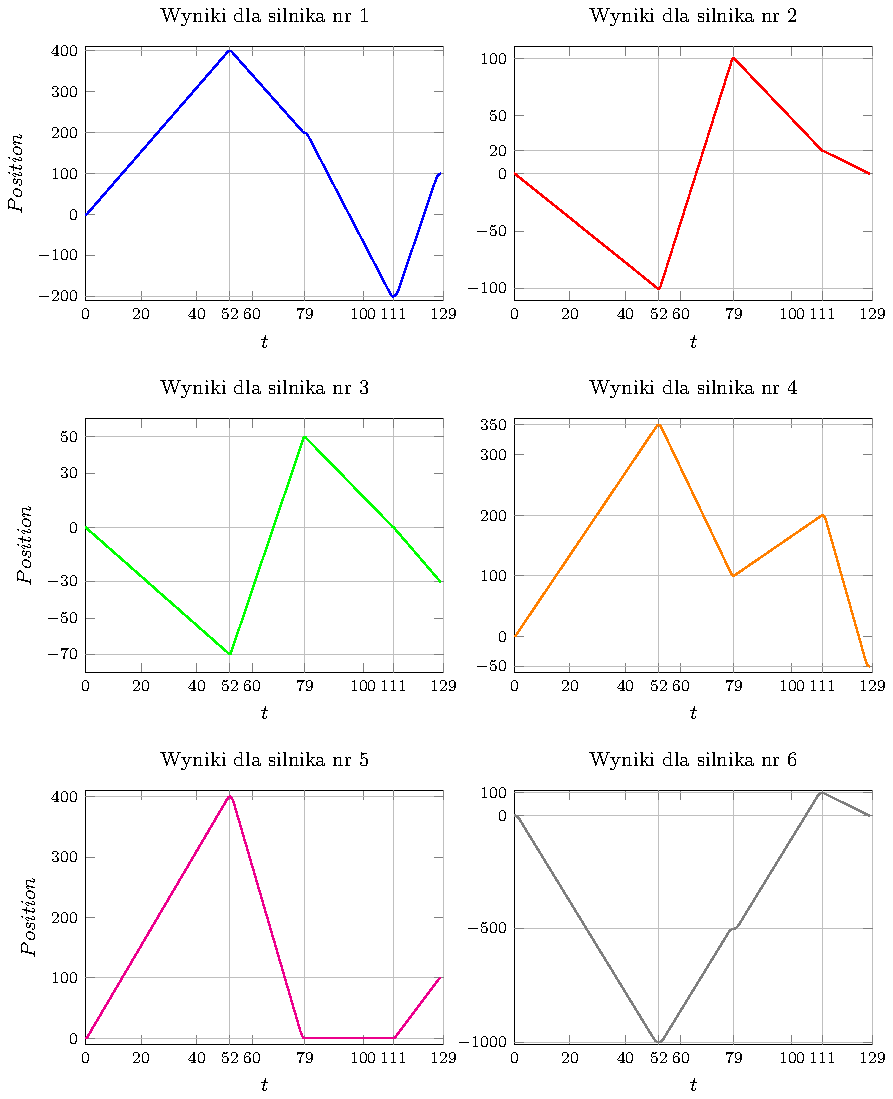
\includegraphics[scale=1.05]{raport_graphs/simpMTDall.pdf}
		\caption{Wyniki testu trajektorii dla wszystkich silników funkcji \texttt{move\_along\_motor\_trajectory\_trapezoid\_duration} przy nastawach z~tablicy \ref{tab:setup11}.}
		\label{fig:simpMTDall}
	\end{figure}
	
	Porównanie wykresów \ref{fig:simpMTDall} z~\ref{fig:simpMTVall}, można z~łatwością zauważyć wydłużenie trajektorii silników, które mogłyby szybciej osiągnąć zadane punkty, lecz zgodnie z założeniami ich ruch trwa tyle ile zajmuje najdłuższa trajektoria.
	
	\subsubsection{Proste działanie w~trybie badawczym}	
	Ponownie nie zauważono różnicy pomiędzy trybami normalnym i~badawczym. Ze względu na udowodnienie działania przy fladze \texttt{research\_mode} ustawionej na \textit{True} w~sekcji \ref{simpMPDR}, pominięto wykresy testów w~tej sekcji.
	
	\begin{table}[H]
	\centering
	\begin{tabular}{|m{2.5em}|m{3em}|m{3.5em}|m{3em}|m{3em}|m{3em}|m{4em}|m{3em}|m{5em}|}
	\hline
	silnik&$ q_i $ & $ q_2 $ & $ q_3 $ & $q_4$ & $ q_f $ & $ v_{max} $ & $ a_{max} $&wynik symulacji\\
	\hline
	\hline
	\hspace{1em}1& 0.0 & 400.0 & 200.0 & -200.0 & 100.0 & 20.0 & 10&\hspace{2em}\checkmark\\ %-400.0144095369332
	\hline
	\hspace{1em}2& 0.0 & -100.0 & 100.0 & 20.0 & 0.0 & 20.0 & 10&\hspace{2em}\checkmark\\ %-100.06421548964671
	\hline
	\hspace{1em}3& 0.0 & -70.0 & 50.0 & 0.0 & -30.0 & 20.0 & 10&\hspace{2em}\checkmark\\ %-70.05025772296632
	\hline
	\hspace{1em}4& 0.0 & 350.0 & 100.0 & 200.0 & -50.0 & 20.0 & 10&\hspace{2em}\checkmark\\  %-8.869543149594518e-13
	\hline
	\hspace{1em}5& 0.0 & 400.0 & 0.0 & 0.0 & 100.0 & 20.0 & 10&\hspace{2em}\checkmark\\  %-70.00006451911138
	\hline
	\hspace{1em}6& 0.0 & -1000.0 & -500.0 & 100.0 & 0.0 & 20.0 & 10&\hspace{2em}\checkmark\\  %-900.0344946730511
	\hline
	\end{tabular}
	\caption{Wyniki symulacji najprostszego przypadku, badanie oddzielnych silników.}
	\label{tab:setup12}
	\end{table}	
	
	\subsection{\texttt{move\_to\_joint\_position\_trapezoid\_velocity}}
	Testowanie funkcji działającej w~przestrzeni stawów w~trybie prędkościowym. Wykresy wyników rozszerzone zostały o~symulację odpowiedniego ruchu silników.
	
	\subsubsection{Proste działanie w~trybie badawczym}	
	\begin{table}[H]
	\centering
	\begin{tabular}{|m{2.5em}|m{4em}|m{4em}|m{4em}|m{4em}|m{4em}|m{4em}|m{5em}|}
	\hline
	silnik&$ q_i $ & $ q_f $ & $ v_i $ & $ v_f $ & $ v_{max} $ & $ a_{max} $&wynik symulacji\\
	\hline
	\hline
	\hspace{1em}1& -0.1006 & -0.4 & 0.0 & 0.0 & 0.30 & 0.20&\hspace{2em}\checkmark\\ %400.01624549348827
	\hline
	\hspace{1em}2& -1.5419 & 100.0 & 0.0 & 0.0 & 0.30 & 0.20&\hspace{2em}\checkmark\\  %100.06493977550167
	\hline
	\hspace{1em}3& 0.0197 & 100.0 & 0.0 & 0.0 & 0.30 & 0.20&\hspace{2em}\checkmark\\ %100.05074855824355
	\hline
	\hspace{1em}4& 1.1335 & 350.0 & 0.0 & 0.0 & 0.30 & 0.20&\hspace{2em}\checkmark\\  %350.03683107162874
	\hline
	\hspace{1em}5& 3.6581 & 400.0 & 0.0 & 0.0 & 0.30 & 0.20&\hspace{2em}\checkmark\\  %400.0004100112147
	\hline
	\hspace{1em}6& -2.7381 & 2000.0 & 0.0 & 0.0 & 0.30 & 0.20&\hspace{2em}\checkmark\\  %2000.0423718337847
	\hline
	\end{tabular}
	\caption{Wyniki symulacji najprostszego przypadku, badanie oddzielnych silników.}
	\label{tab:simpJPV}
	\end{table}
	
	\begin{table}[H]
	\centering
	\begin{tabular}{|m{2.5em}|m{4em}|m{4em}|m{4em}|m{4em}|m{4em}|m{4em}|m{5em}|}
	\hline
	silnik&$ q_i $ & $ q_f $ & $ v_i $ & $ v_f $ & $ v_{max} $ & $ a_{max} $&wynik symulacji\\
	\hline
	\hline
	\hspace{1em}1& 0.0 & -400.0 & 0.0 & 0.0 & 25.0 & 10&\hspace{2em}\checkmark\\ %-400.0162154089848
	\hline
	\hspace{1em}2& 0.0 & -100.0 & 0.0 & 0.0 & 35.0 & 20&\hspace{2em}\checkmark\\ %-100.06384704599024
	\hline
	\hspace{1em}3& 0.0 & -70.0 & 0.0 & 0.0 & 35.0 & 20&\hspace{2em}\checkmark\\ %-70.04977729182792
	\hline
	\hspace{1em}4& 0.0 & -60.0 & 0.0 & 0.0 & 35.0 & 20&\hspace{2em}\checkmark\\  %-60.036372838521224
	\hline
	\hspace{1em}5& 0.0 & -70.0 & 0.0 & 0.0 & 35.0 & 20&\hspace{2em}\checkmark\\  %-70.00005703129563
	\hline
	\hspace{1em}6& 0.0 & -900.0 & 0.0 & 0.0 & 35.0 & 20&\hspace{2em}\checkmark\\  %-900.0418019049634
	\hline
	\end{tabular}
	\caption{Wyniki symulacji najprostszego przypadku, badanie oddzielnych silników.}
	\label{tab:simpJPVrevers}
	\end{table}

	\begin{figure}[H]
		\centering
		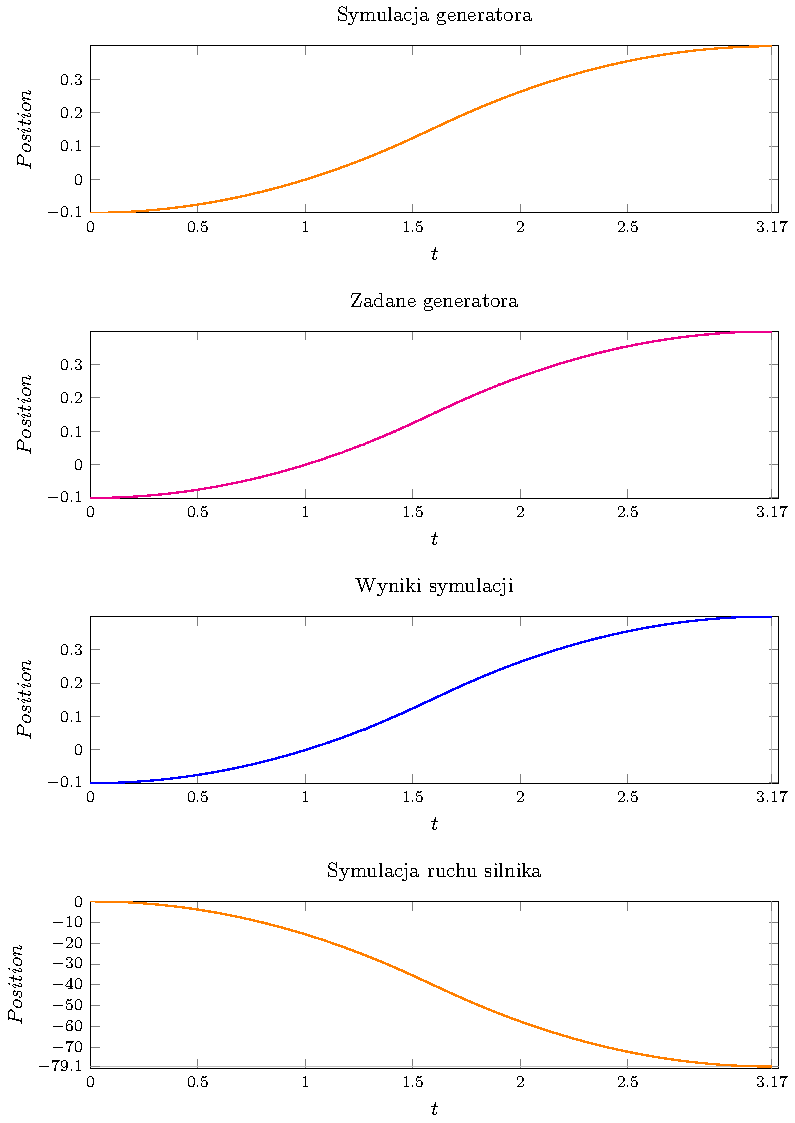
\includegraphics[scale=1.2]{raport_graphs/simpJPV.pdf}
		\caption{Wyniki testu trajektorii dla silnika pierwszego funkcji \texttt{move\_to\_motor\_position\_trapezoid\_velocity} przy nastawach z~tablicy \ref{tab:simpJPV}.}
		\label{fig:simpJPV}
	\end{figure}


	\begin{figure}[H]
		\centering
		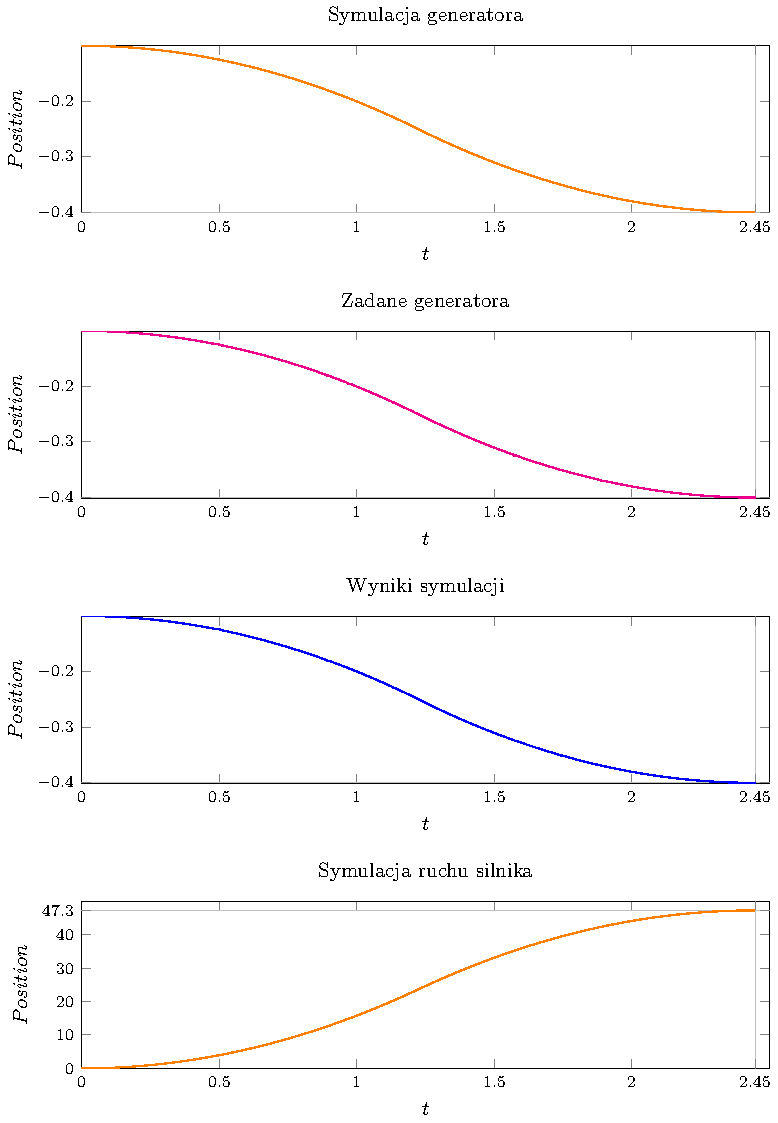
\includegraphics[scale=1.2]{raport_graphs/simpJPVrevers.pdf}
		\caption{Wyniki testu trajektorii dla silnika pierwszego funkcji \texttt{move\_to\_motor\_position\_trapezoid\_velocity} przy nastawach z~tablicy \ref{tab:simpJPVrevers}.}
		\label{fig:simpJPVrevers}
	\end{figure}
		
	\begin{figure}[H]
		\centering
		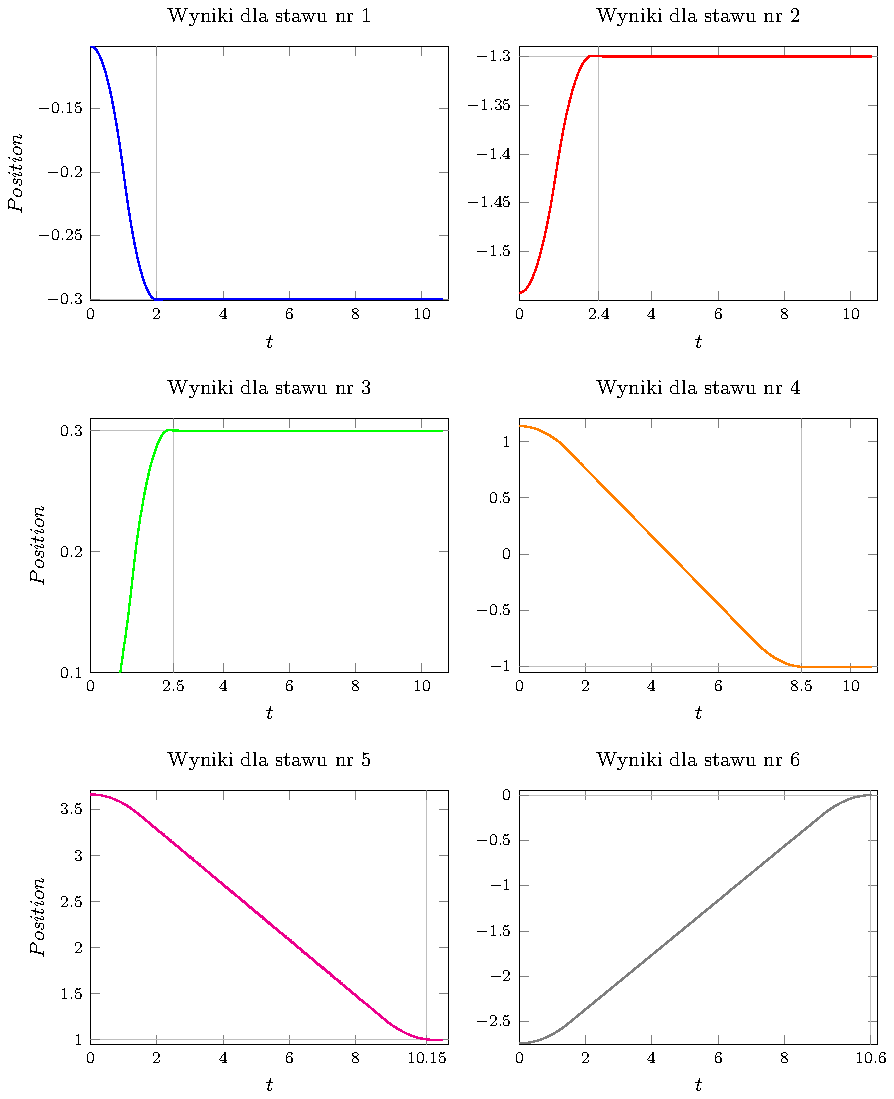
\includegraphics[scale=1.1]{raport_graphs/simpJPVall.pdf}
		\caption{Wyniki testu trajektorii dla silnika pierwszego funkcji \texttt{move\_to\_motor\_position\_trapezoid\_velocity} przy nastawach z~tablicy \ref{tab:simpJPV}.}
		\label{fig:simpJPVall}
	\end{figure}
	
	
\newpage	
\begin{thebibliography}{9}
\bibitem{ROS} 
Dokumentacja pakietu actionlib

http://wiki.ros.org/actionlib, Open Source Robotics Fundation, kwiecień 2018.

\bibitem{jtm} 
Dokumentacja wiadomości trajectory\_msgs/JointTrajectory

http://docs.ros.org/api/trajectory\_msgs/html/msg/JointTrajectory.html, Open Source Robotics Fundation, maj 2018.

\bibitem{cmjtm} 
Dokumentacja wiadomości control\_msgs/JointTolerance.msg

http://docs.ros.org/jade/api/control\_msgs/html/msg/JointTolerance.html, Open Source Robotics Fundation, luty 2016.

\bibitem{jtpm}
Dokumentacja wiadomości trajectory\_msgs/JointTrajectoryPoint.msg

http://docs.ros.org/api/trajectory\_msgs/html/msg/JointTrajectoryPoint.html, Open Source Robotics Fundation, maj 2018.

\bibitem{orocosbuild} 
The Orocos Component Builder's Manual

 http://www.orocos.org/stable/documentation/rtt/v2.x/doc-xml/orocos-components-manual.html, Open RObot COntrol Software, 2012.
\end{thebibliography}	
	
\end{document}




}